% Slide1: Introduction -----------------------------------------------------------



\begin{frame}
  \frametitle{The Reco Problem Revisited}
 
 
   \begin{figure}[h!]
     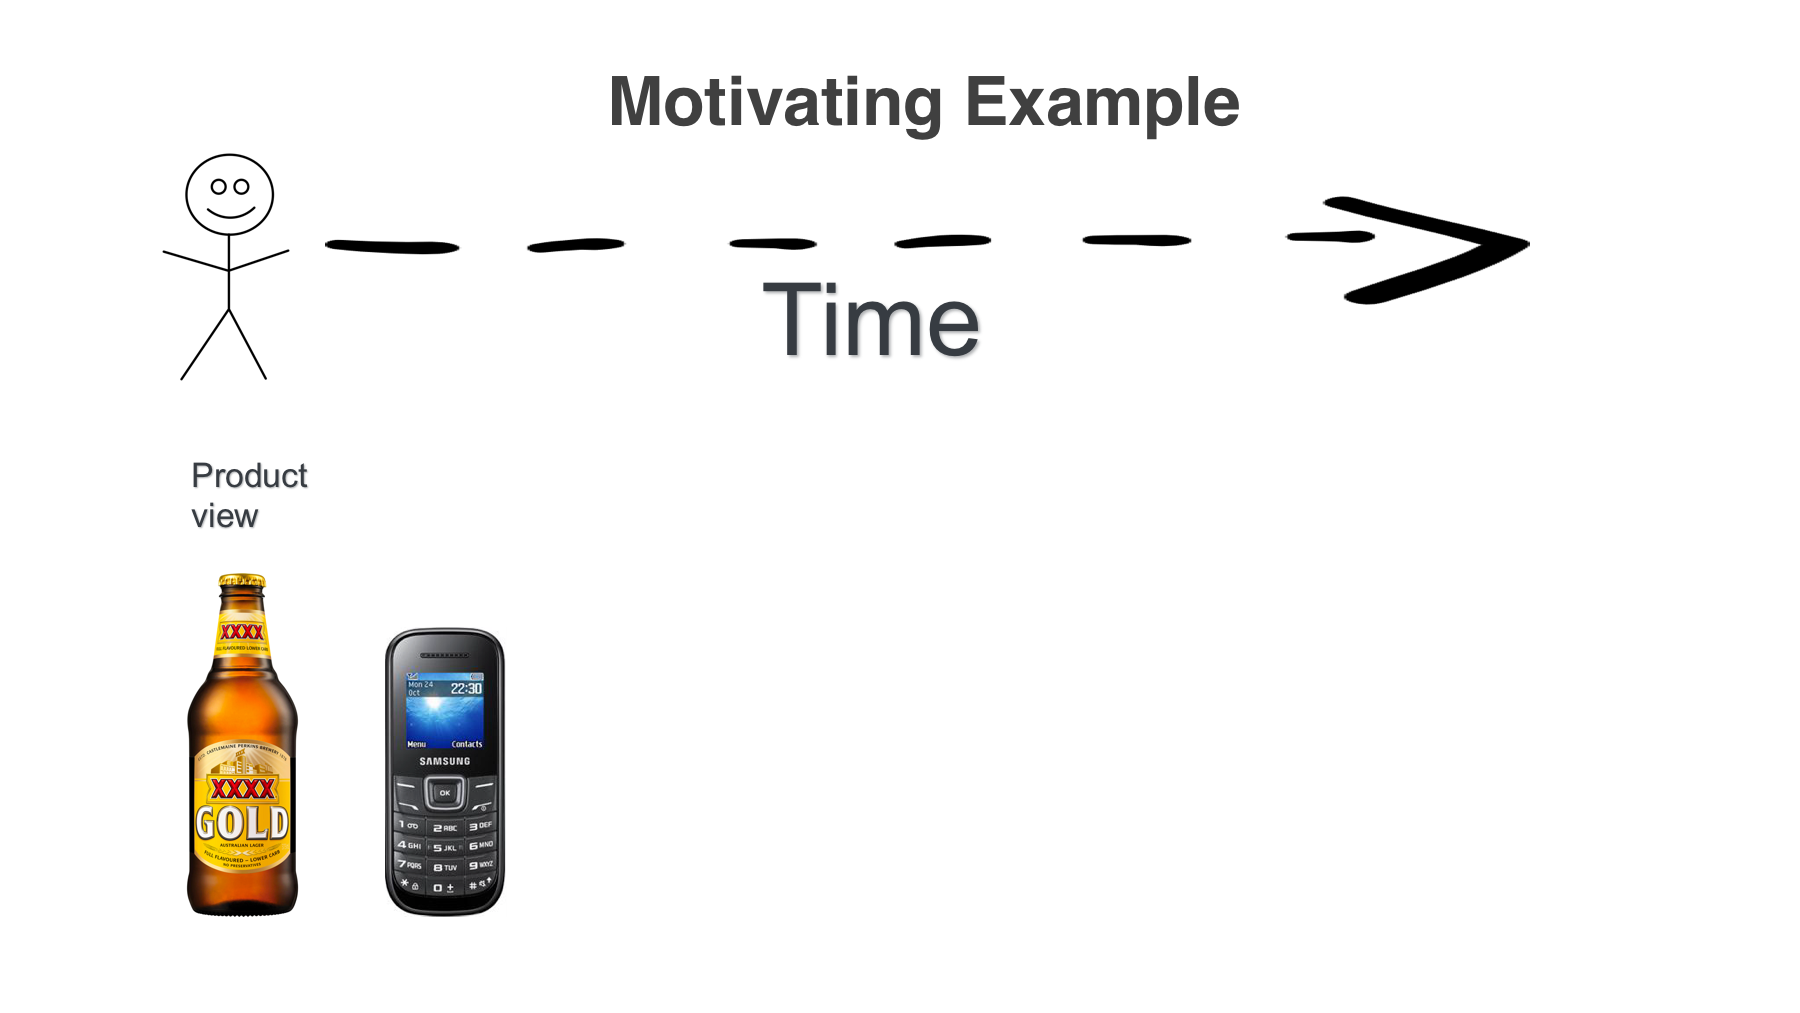
\includegraphics[scale=0.3]{images/mot_ex1.png}
       \centering
       \label{motex1}
   \end{figure}
     
 \end{frame}



 \begin{frame}
  \frametitle{The Reco Problem Revisited}
 
 
   \begin{figure}[h!]
     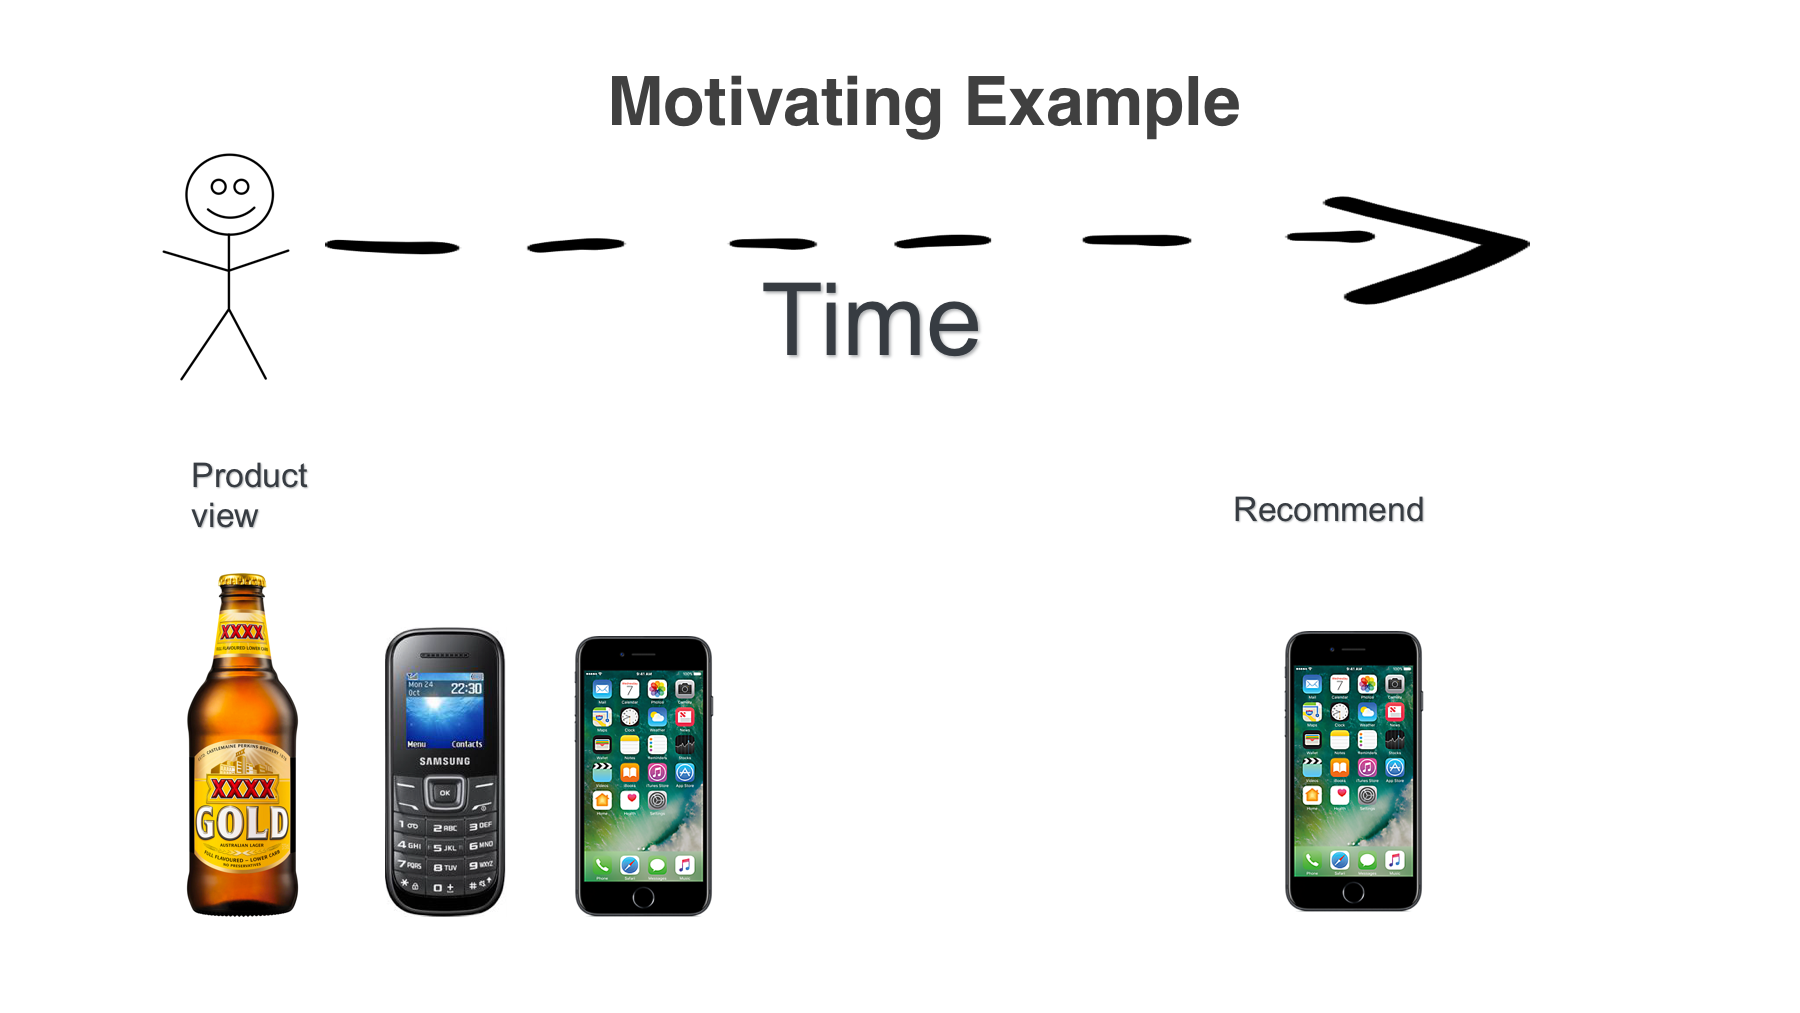
\includegraphics[scale=0.3]{images/mot_ex2.png}
       \centering
       \label{motex1}
   \end{figure}
     
 \end{frame}

 \begin{frame}
  \frametitle{The Reco Problem Revisited}
 
 
   \begin{figure}[h!]
     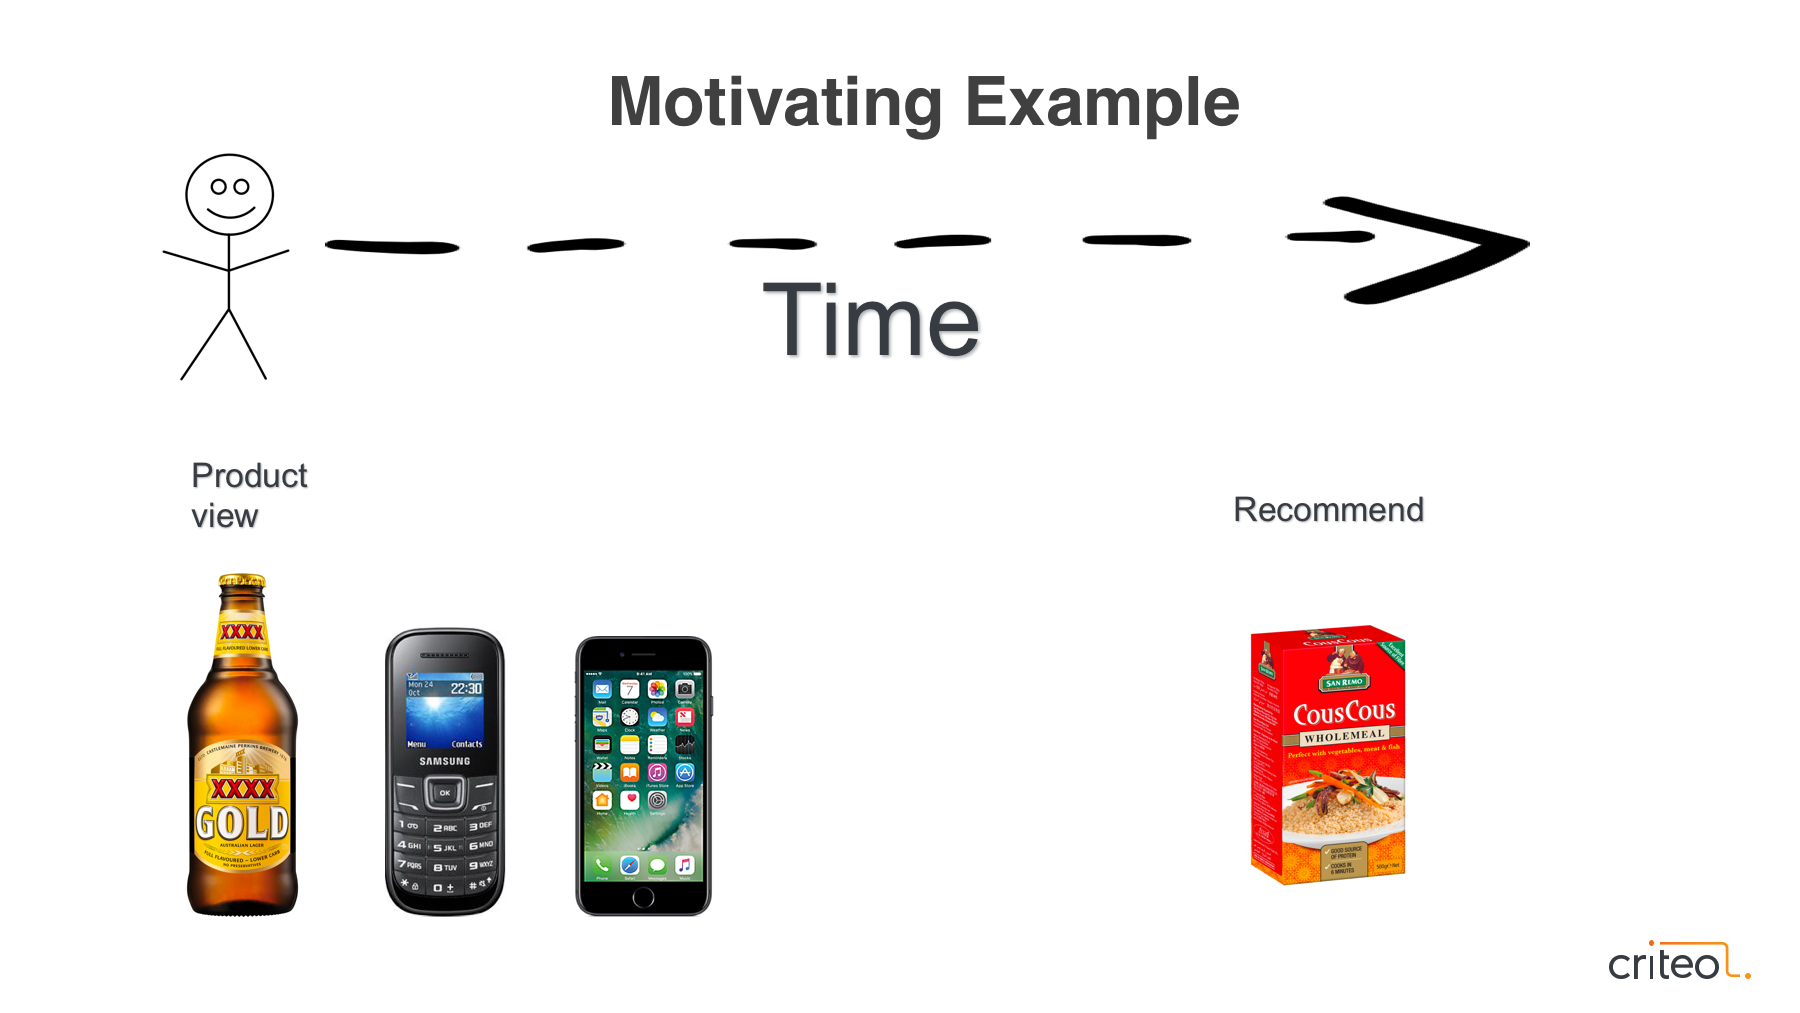
\includegraphics[scale=0.3]{images/mot_ex3.png}
       \centering
       \label{motex1}
   \end{figure}
     
 \end{frame}

 \begin{frame}
  \frametitle{The Reco Problem Revisited}
 
 
   \begin{figure}[h!]
     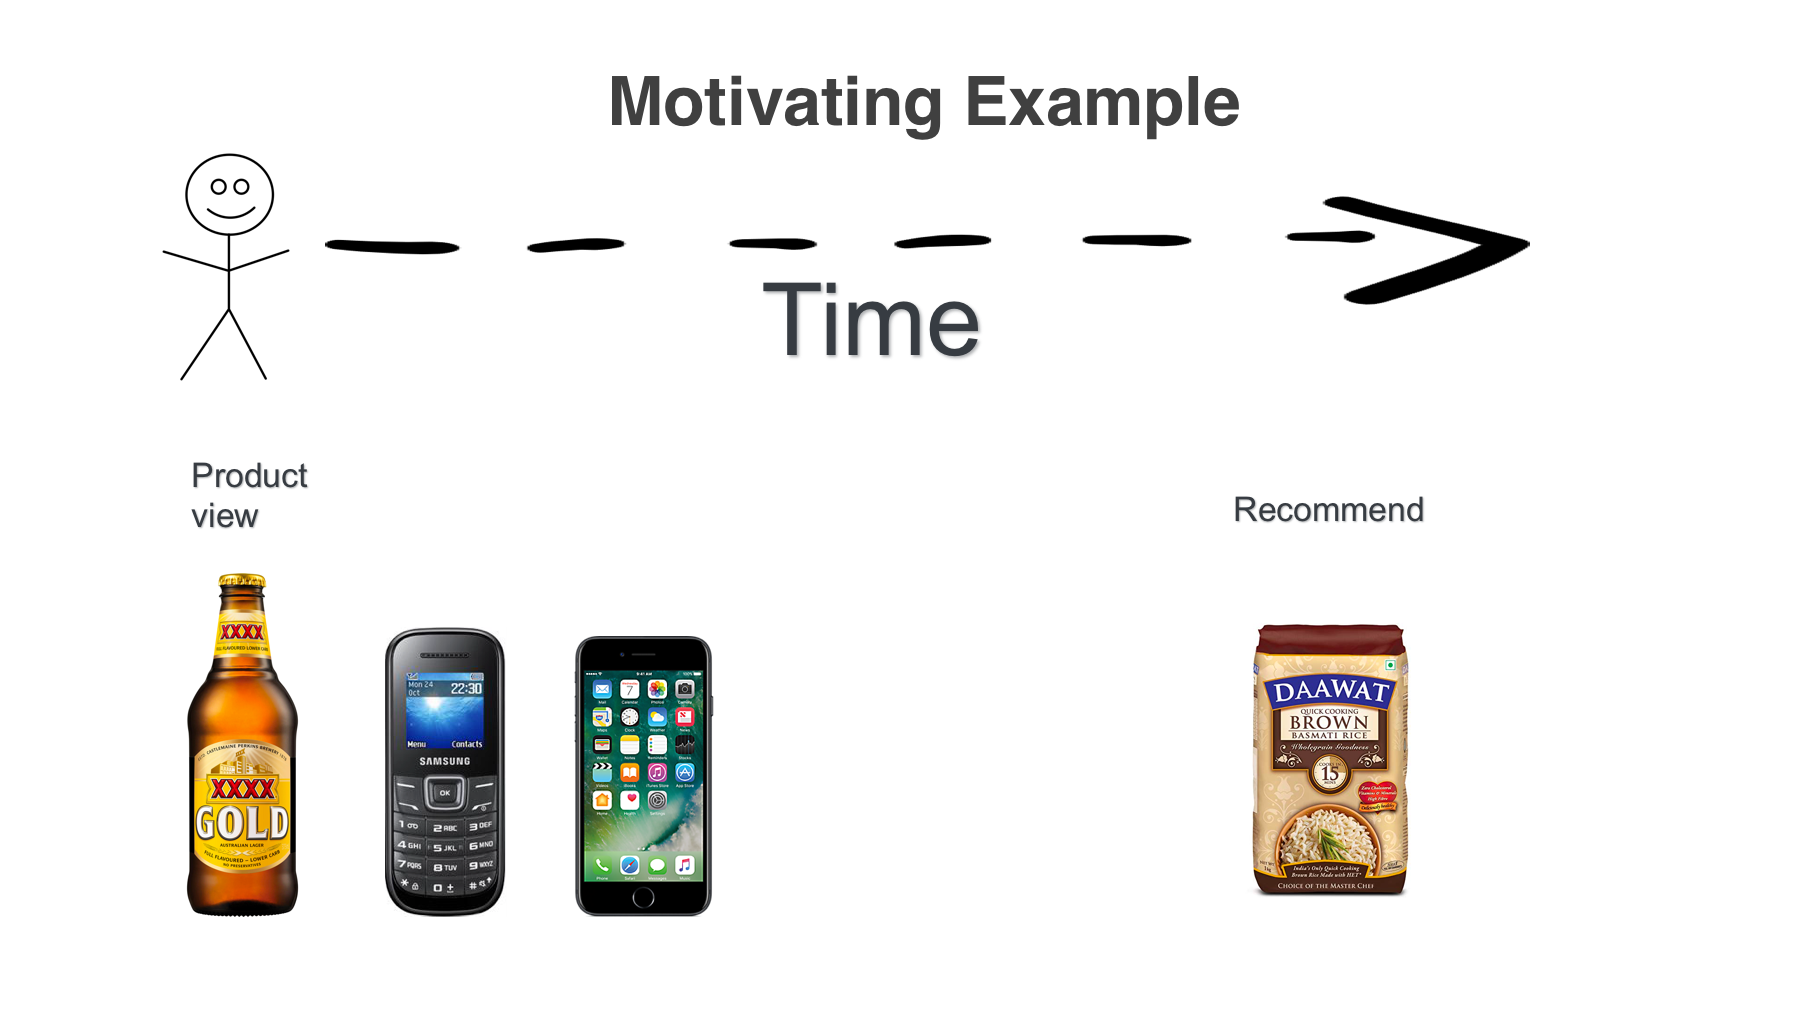
\includegraphics[scale=0.3]{images/mot_ex4.png}
       \centering
       \label{motex1}
   \end{figure}
     
 \end{frame}



 \begin{frame}
  \frametitle{The Reco Problem Revisited}
 
 
   \begin{figure}[h!]
     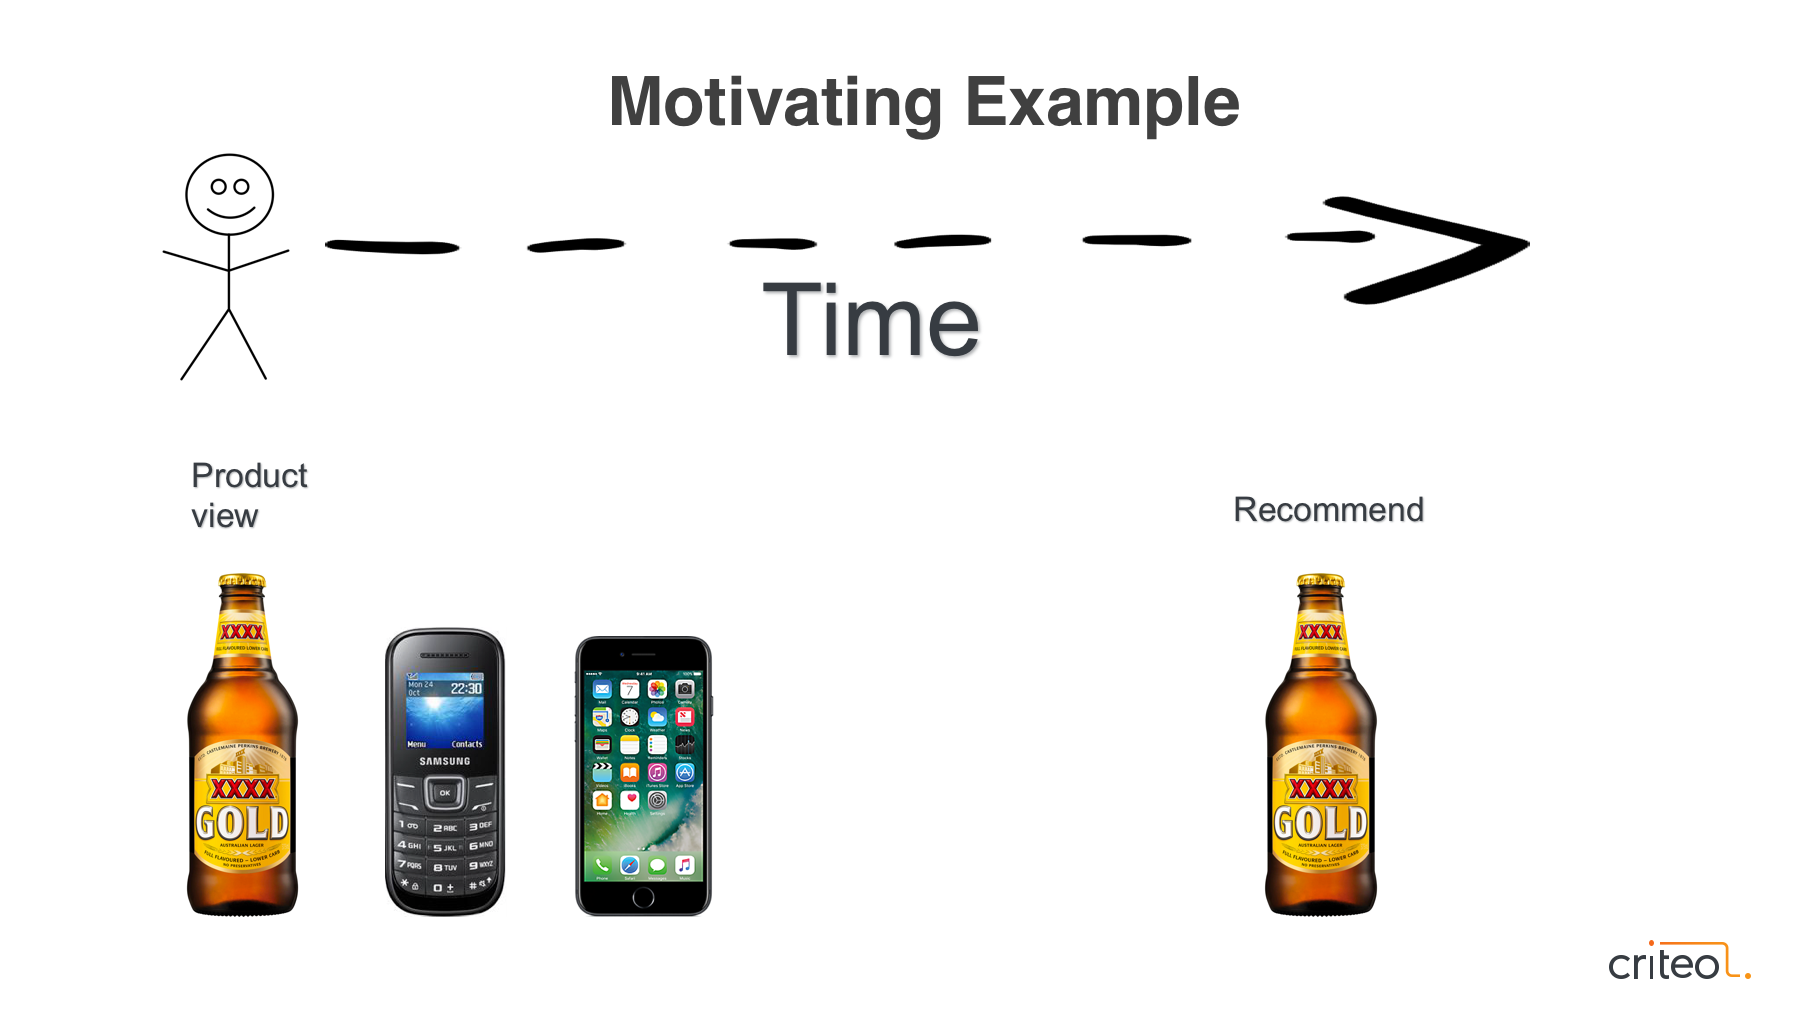
\includegraphics[scale=0.3]{images/mot_ex5.png}
       \centering
       \label{motex1}
   \end{figure}
     
 \end{frame}

 \begin{frame}
  
   \begin{figure}[h!]
     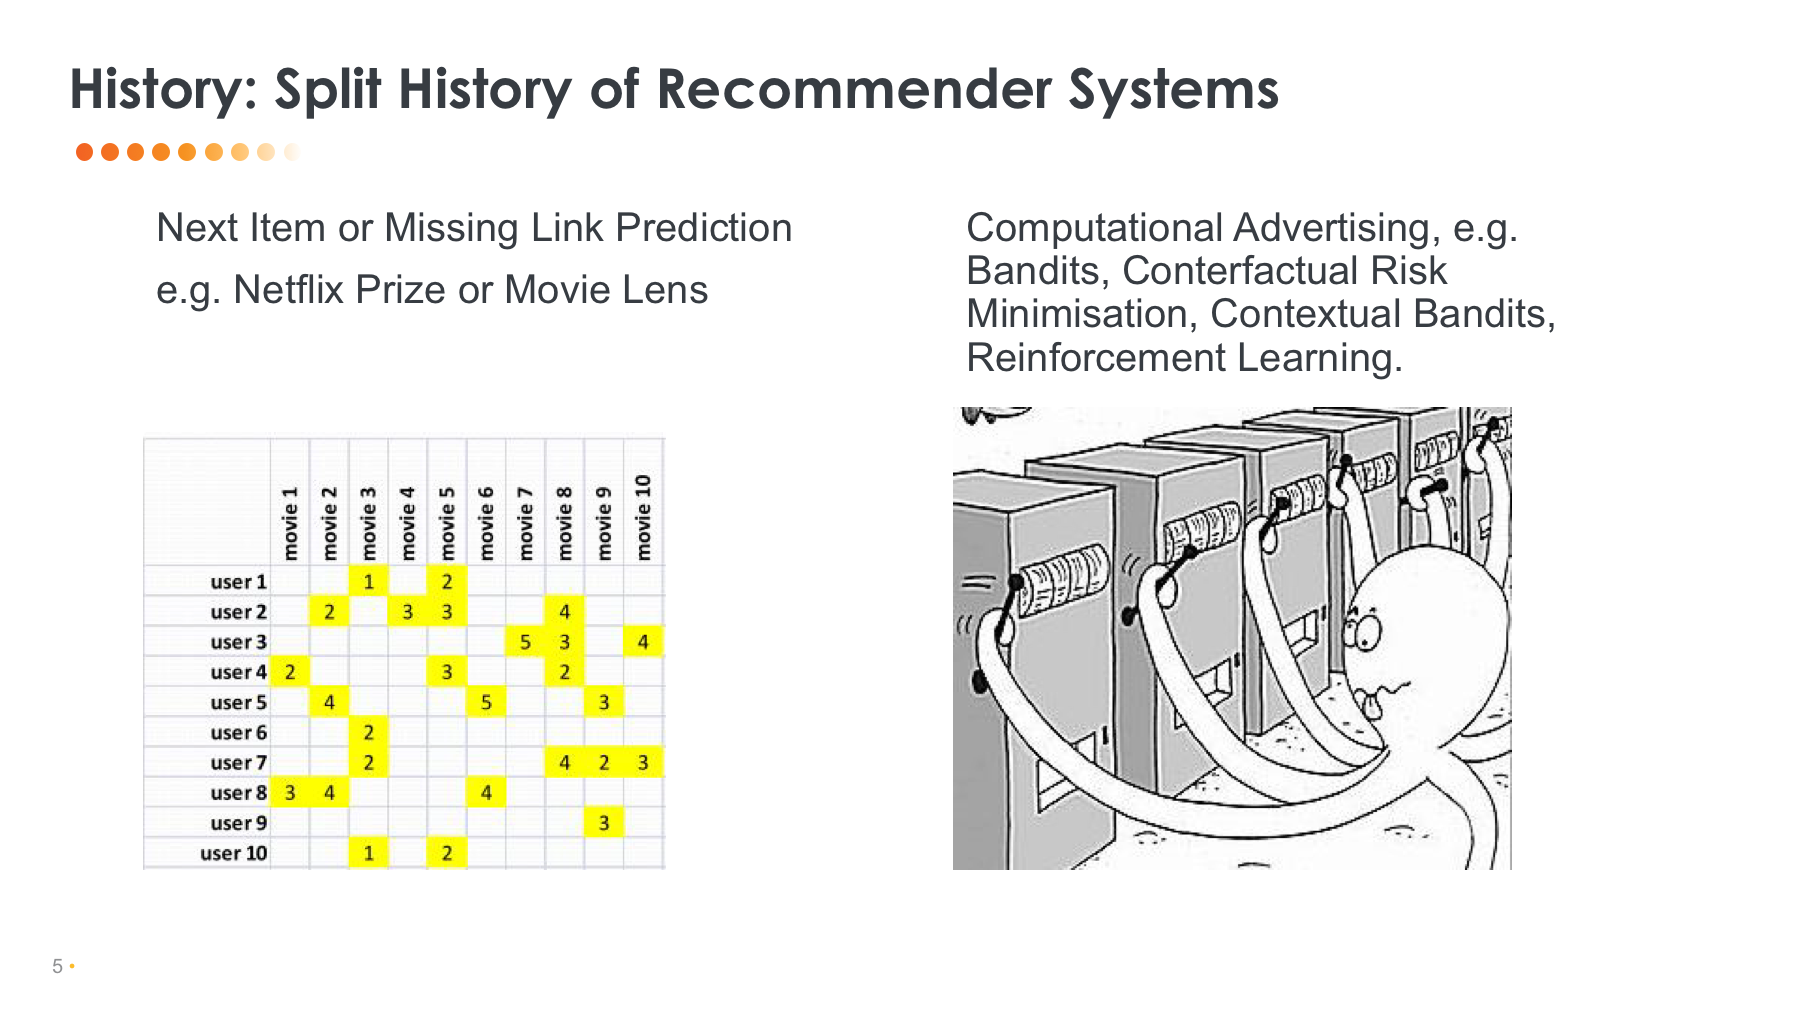
\includegraphics[scale=0.34]{images/octo.png}
       \centering
       \label{motex1}
   \end{figure}
     
 \end{frame}


 \begin{frame}
  \frametitle{Classic RecSys Datasets: Are they logs of recommender systems?}

  \begin{itemize}
    \item MovieLens: \pause no, explicit feedback of movie ratings \pause
    \item Netflix Prize: \pause no, explicit feedback of movie ratings \pause
    \item Yoochoose (RecSys 15): \pause no, implicit session based behavior \pause
    \item 30 Music: \pause no, implicit session based behavior \pause
    \item Criteo Dataset for counterfactual evaluation of RecSys algorithms: \pause yes!
  \end{itemize}

  \pause
  The Criteo Dataset shows a log of recommendations and if they were successful in getting users to click.  
\end{frame}



\begin{frame}
  \frametitle{Classic RecSys Evaluation Metrics: Do they evaluate the quality of recommendation?}

  \begin{itemize}
    \item Recall@K, Precision@K, HR@K:  \pause no, evaluates next item prediction \pause
    \item DCG:   \pause no, evaluates next item prediction \pause
    \item Log likelihood: \pause  unclear, but ususally next item prediction \pause
    \item Inverse Propensity Score estimate of click through rate: \pause yes! (although it is often noisy) \pause
    \item AB Test: \pause yes, but the academic literature has no access to this
  \end{itemize}

  \pause
If the dataset does not contain a log of recommendations and if they were successful, you cannot compute metrics of the recommendation quality.
\end{frame}


\begin{frame}
  \frametitle{Let's take a step back...}
  
  \textbf{How are we improving large-scale Recommender Systems in the Real World}
  
  \begin{itemize}
  \item Learn a supervised model from past user activity
  \item Evaluate offline and decide whether to A/B test
  \item A/B test
  \item If positive and scalable, roll-out
  \item If not, try to understand what happened and try to create a better model of the world using the same past data
  \item Repeat
  \end{itemize}
        
  \end{frame}
  



  
  
  
  \begin{frame}
    \frametitle{Supervised learning with the wrong objective}
  
  Most of the time, we frame the problem either as:
  \begin{itemize}
  \item Missing link prediction
  \item Next user event prediction
  \end{itemize}
  
  \end{frame}
  
  
  \begin{frame}
    \frametitle{Supervised learning with the wrong objective}
  
  We are operating under the assumption that the best recommendation policy is in some sense the \textbf{optimal auto-complete of natural user behavior}
  
  \end{frame}
  
  
  \begin{frame}
    \frametitle{Supervised learning with the wrong objective}
  
  From the point of view of business metrics, \textbf{learning to autocomplete behavior is a great initial recommendation policy}, especially when no prior user feedback is available. 
  
  \end{frame}
  
  
  \begin{frame}
    \frametitle{Supervised learning with the wrong objective}
  
  \textbf{However}, after a first golden age, where all offline improvements turn into positive A/B tests, the \emph{naive recommendation} optimization objective and the business objective will start to diverge.
  
  \end{frame}
  
  
  \begin{frame}
    \frametitle{Aligning the Recommendation objective with the business}
  
  \begin{itemize}
  \item Of course, we could start incorporating user feedback that we collected while running the initial recommendation policies  
  \item We should be able to continue bringing improvements using feedback that is now aligned with our business metrics (ad CTR, post click sales, dwell time, number of videos watched, ...)
  \end{itemize}
  
  \end{frame}
  
  
  \begin{frame}
    \frametitle{Aligning the Recommendation objective with the business}
  
    However, this does not come without caveats...
  
  \end{frame}
  
  
  \begin{frame}
    \frametitle{Recommendation as Supervised Learning and AB Testing}
   
   
     \begin{figure}[h!]
       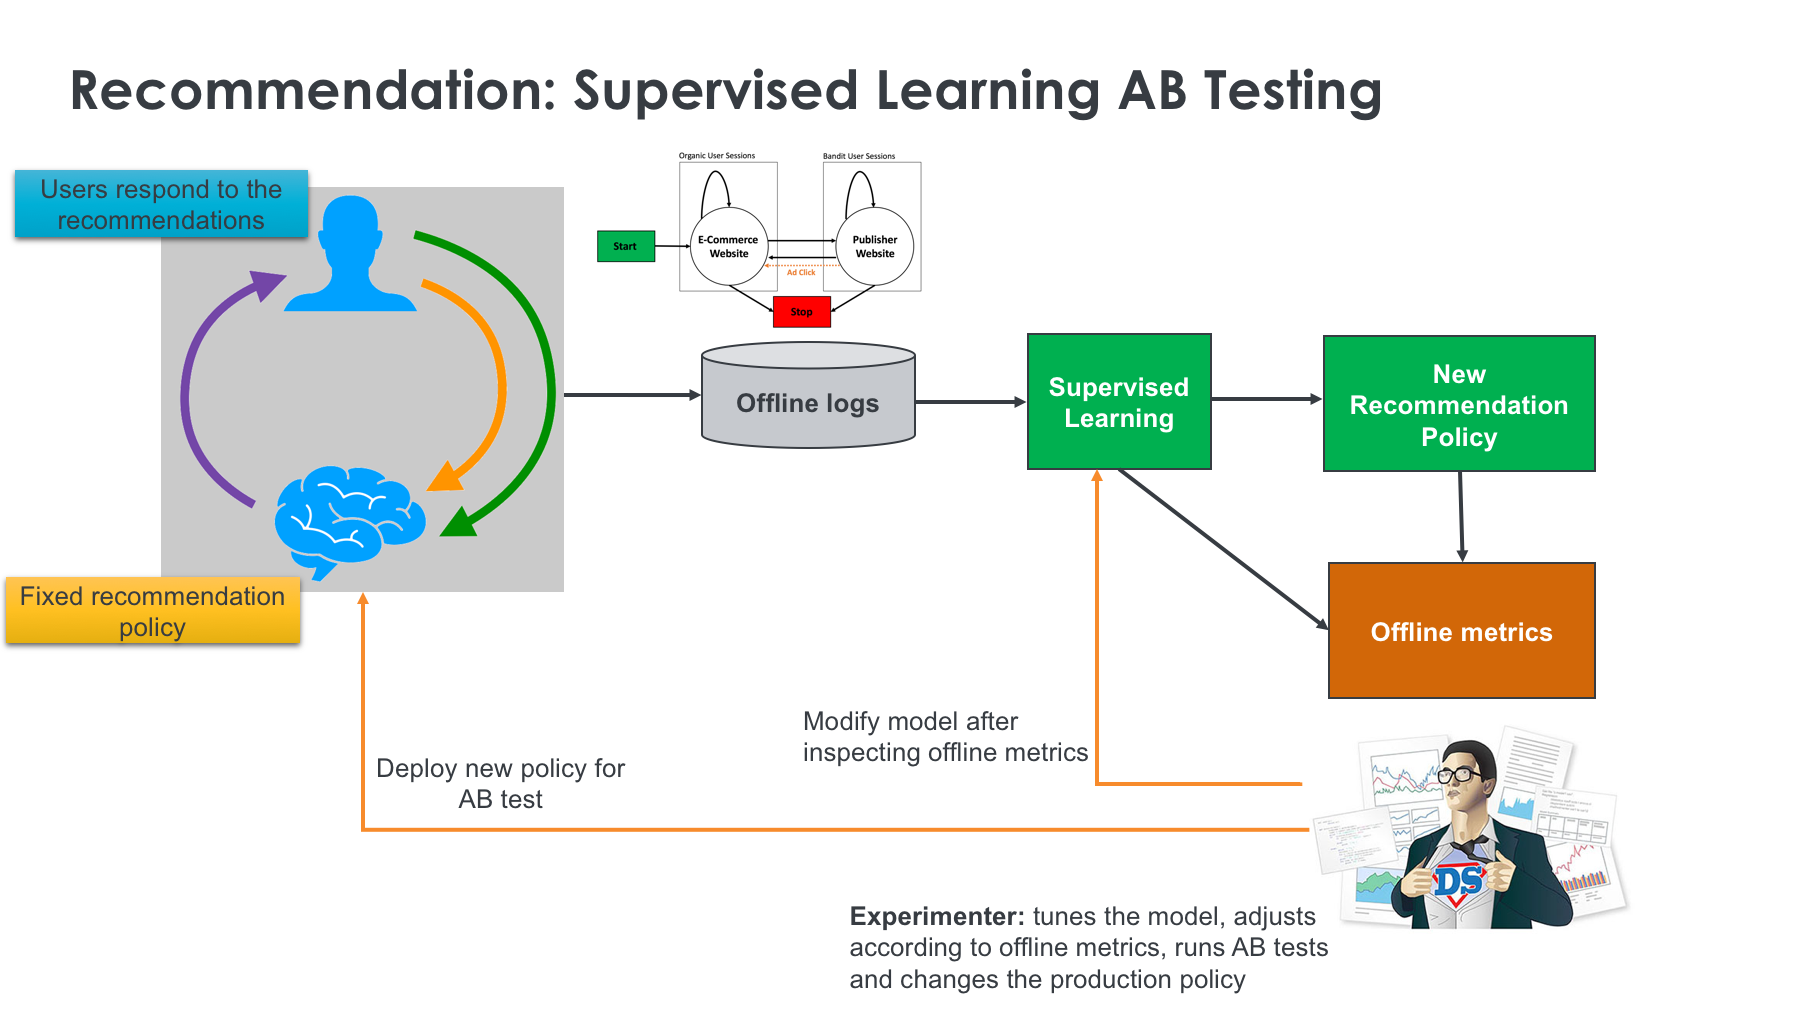
\includegraphics[scale=0.3]{images/recoasabtesting0.png}
         \centering
         \label{motex1}
     \end{figure}
       
   \end{frame}
  
        


 \begin{frame}
  \frametitle{Recommendation as Supervised Learning and AB Testing}
 
 
   \begin{figure}[h!]
     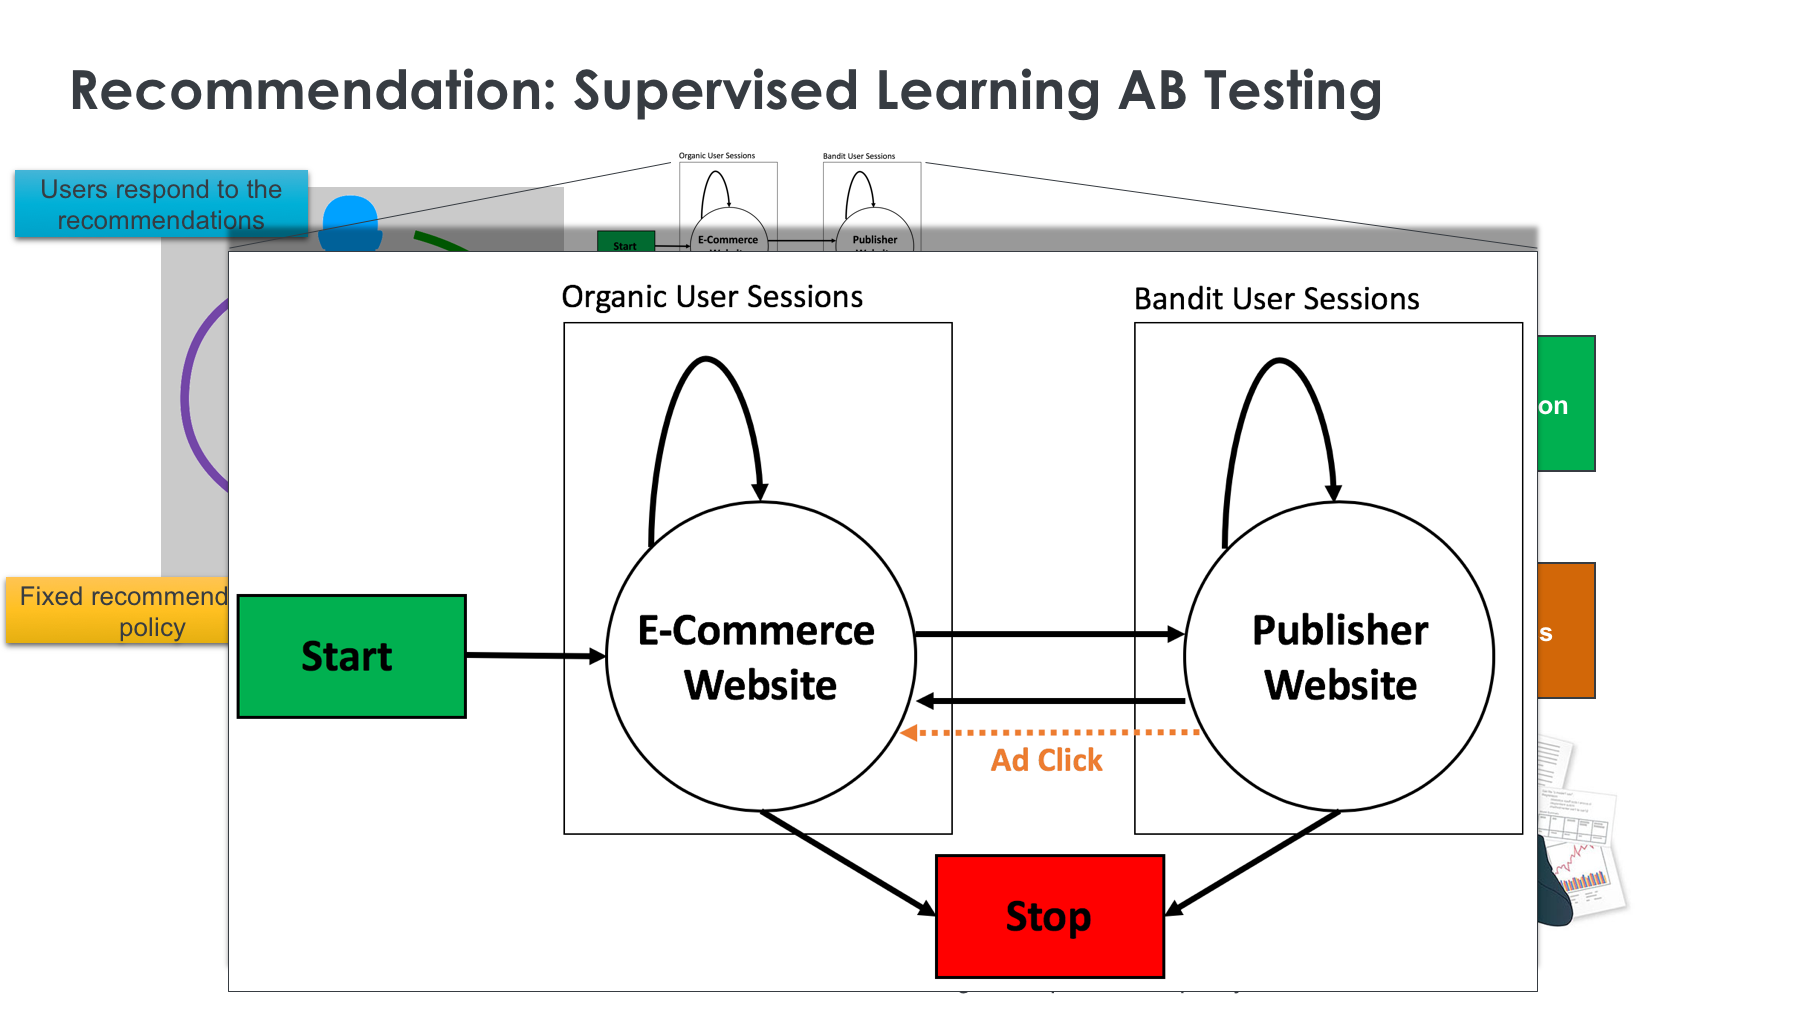
\includegraphics[scale=0.3]{images/recoasabtesting.png}
       \centering
       \label{motex1}
   \end{figure}
     
 \end{frame}





 
\begin{frame}
  \frametitle{Modern Recommendation Systems Research}
  
  \textbf{Q: How does the literature on Large Scale Recommendation Systems look right now?}
  
  A: Most of the latest publications are talking about ways of using Deep Learning for Recommendation:
  \begin{itemize}
  \item \textbf{Matrix Factorization extensions:} Word2Vec, Deep and Wide, Neural MF, Node2Vec 
  \item \textbf{Content-based recommendation:} CNNs for Image, Text, Sounds to compute item similarities
  \item \textbf{Next event prediction / user activity modeling:} RNNs, TCNs
  \end{itemize}
  
\end{frame}


\begin{frame}
  \frametitle{Modern Recommendation Systems Research}
  
  \textbf{We see great improvements in offline metrics!}
  
  \begin{itemize}
  \item \textbf{Regression/Classification metrics:} MSE, AUC, NLL
  \item \textbf{Ranking metrics:} MPR, Precision@k, NDCG
  \end{itemize}
  
\end{frame}


\begin{frame}
  \frametitle{What is wrong with this picture?}
  
	\textbf{In the same time, as practitioners, we see difficulties in improving the Real World Recommendation models!}

	Offline - online metrics alignment for recommendation is a recognized problem:
	\begin{itemize}
	\item \textbf{Previous work:} Missing Not At Random (MNAR) framework for Matrix factorization, Bandits Literature
	\item \textbf{New avenues:}  \emph{REVEAL: Offline evaluation for recommender systems Workshop at RecSys 2019} (this September in Copenhagen) \url{https://recsys.acm.org/recsys19/reveal/}
	\end{itemize}
  
\end{frame}


\begin{frame}
  \frametitle{The relationship between Reinforcement Learning and Recommendation}

\begin{itemize}
\item We are doing Reinforcement Learning by hand!
\pause
\item Furthermore, we are trying to do RL using the Supervised Learning Framework
\pause
\item Standard test data sets do not let us explore this aspect of recommender systems
\end{itemize}

\pause
.. but how do you evaluate a reinforcement learning algorithm?
\end{frame}

  



\begin{frame}
  \frametitle{}
 
 
   \begin{figure}[h!]
     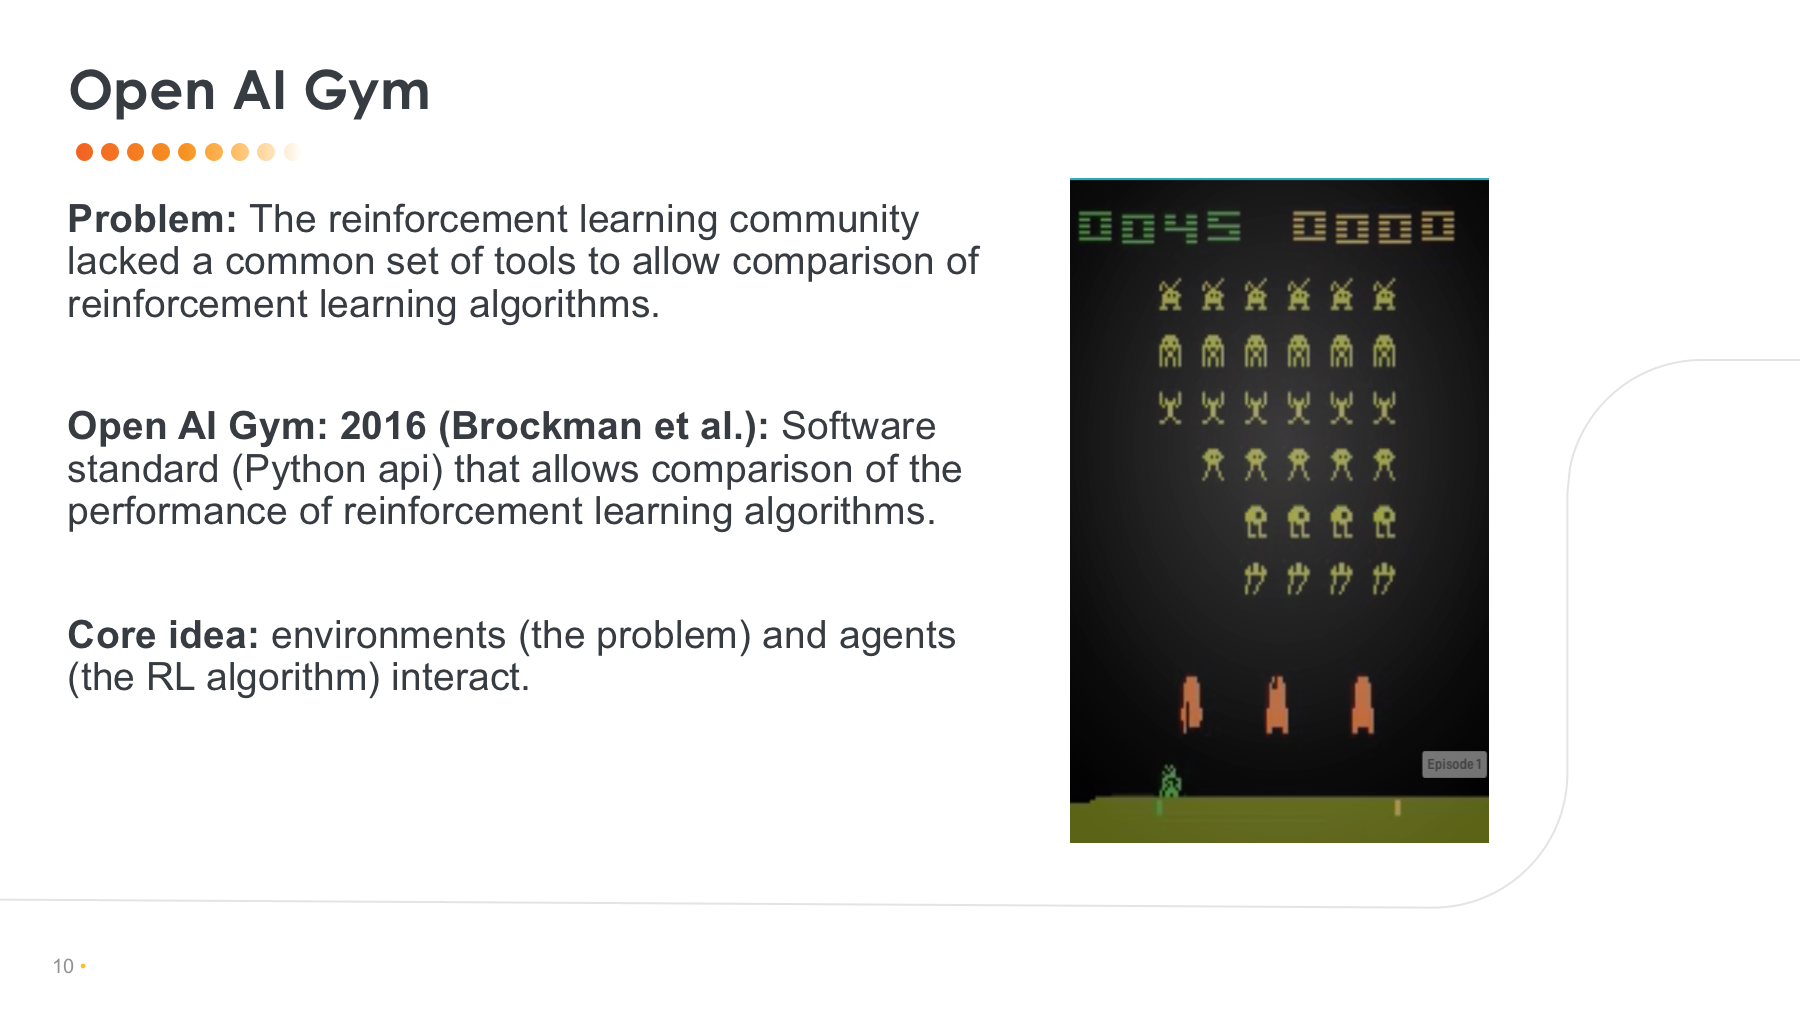
\includegraphics[scale=0.39]{images/openai.png}
       \centering
       \label{motex1}
   \end{figure}
     
 \end{frame}



 \begin{frame}
  \frametitle{}
 
 
   \begin{figure}[h!]
     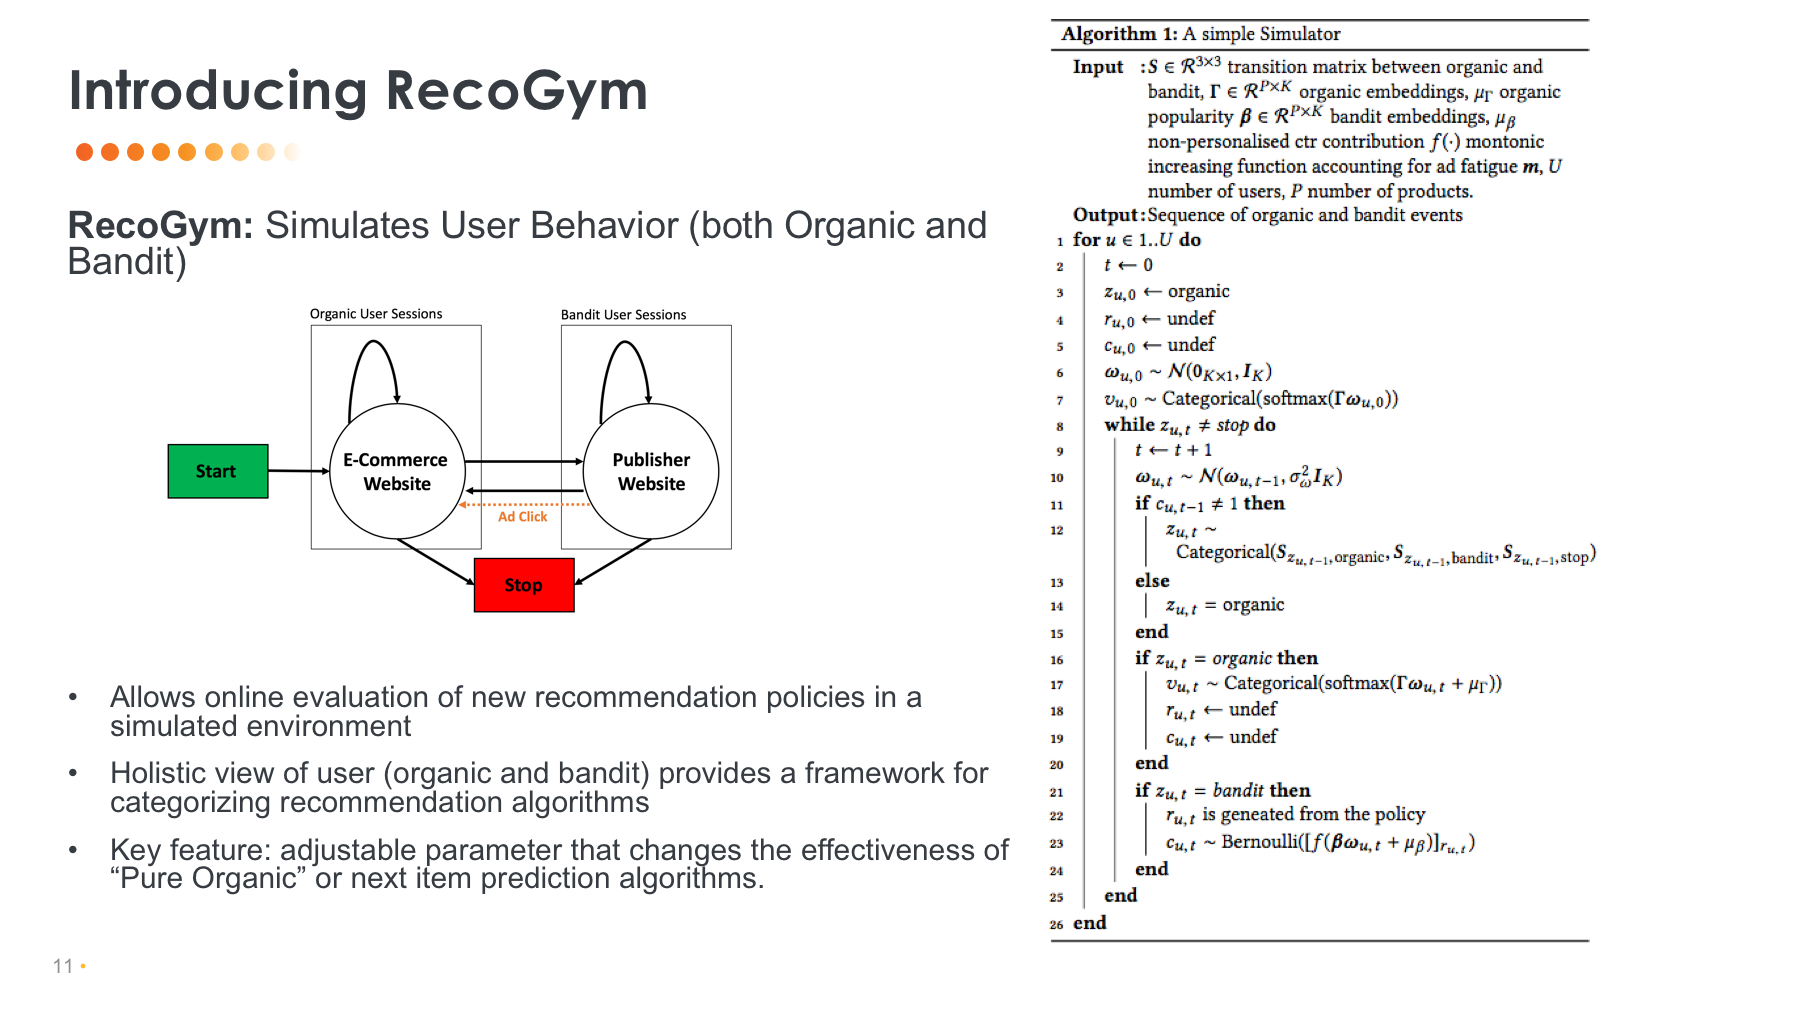
\includegraphics[scale=0.34]{images/recogym1}
       \centering
       \label{motex1}
   \end{figure}
     
 \end{frame}





 \begin{frame}
  \frametitle{}
 
 
   \begin{figure}[h!]
     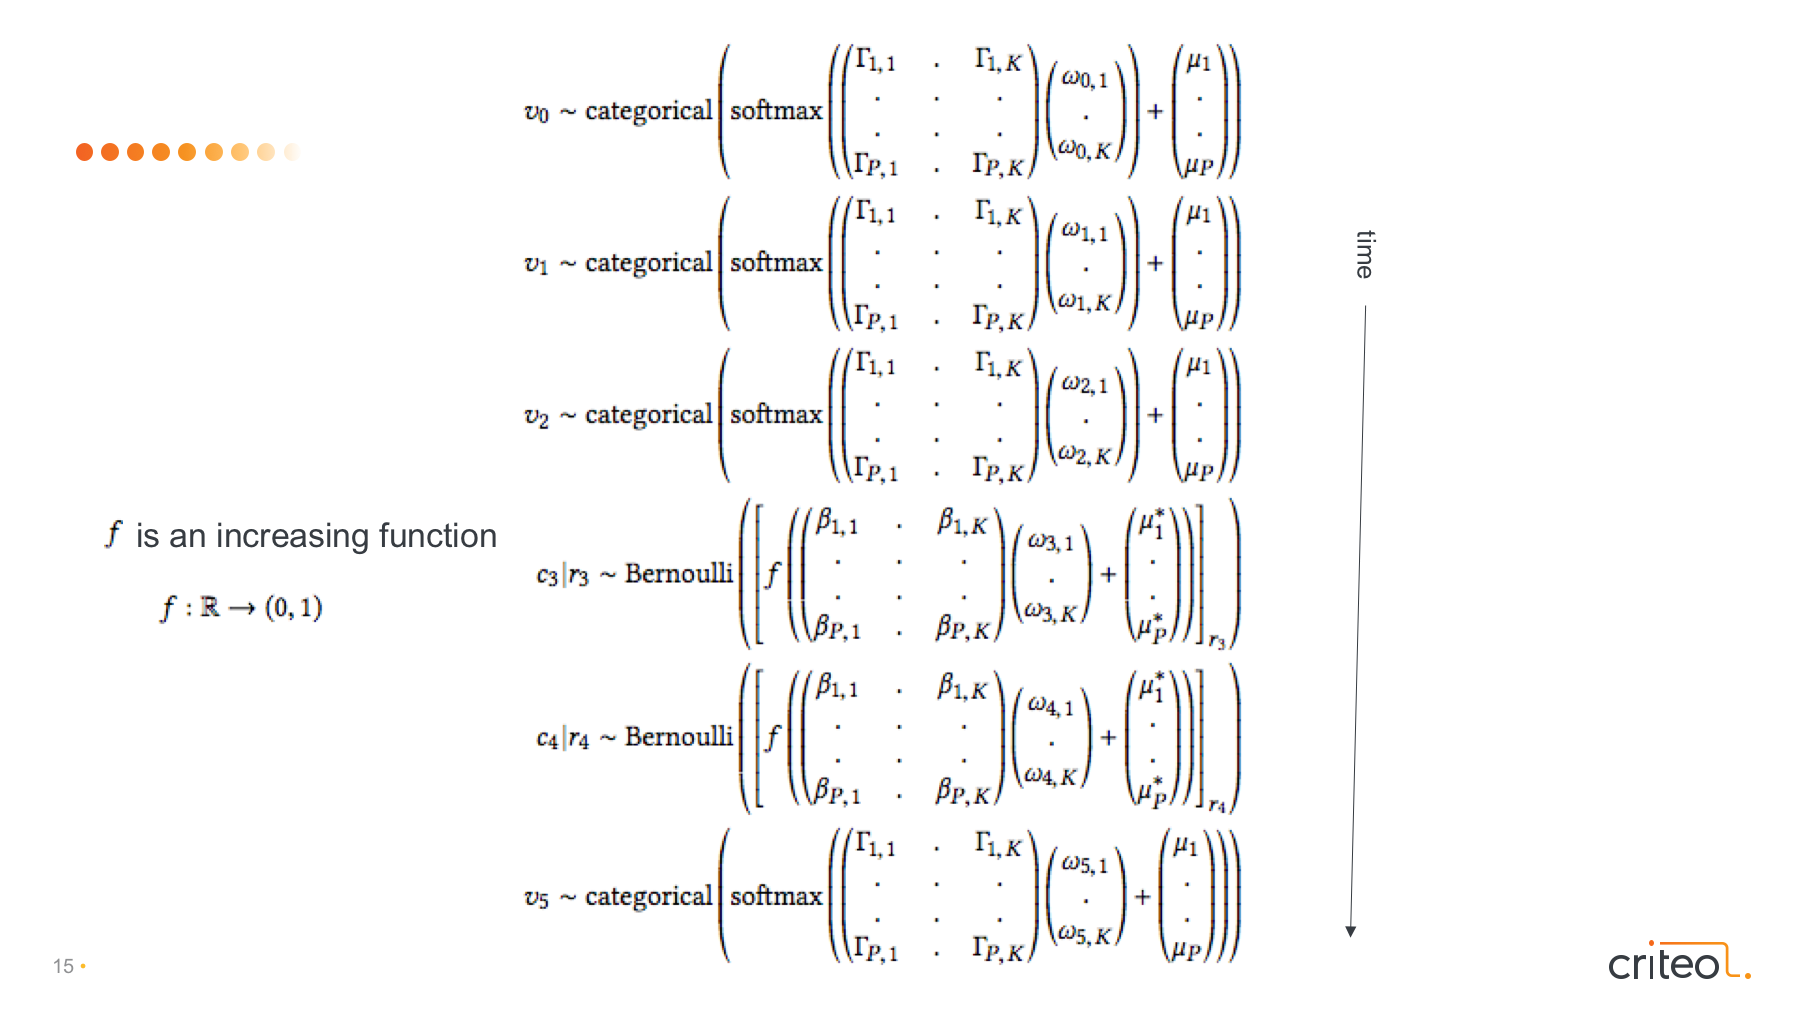
\includegraphics[scale=0.3]{images/recogymsim}
       \centering
       \label{motex1}
   \end{figure}
     
 \end{frame}



 \begin{frame}
  \frametitle{The RecoGym Session}
 
 
   \begin{figure}[h!]
     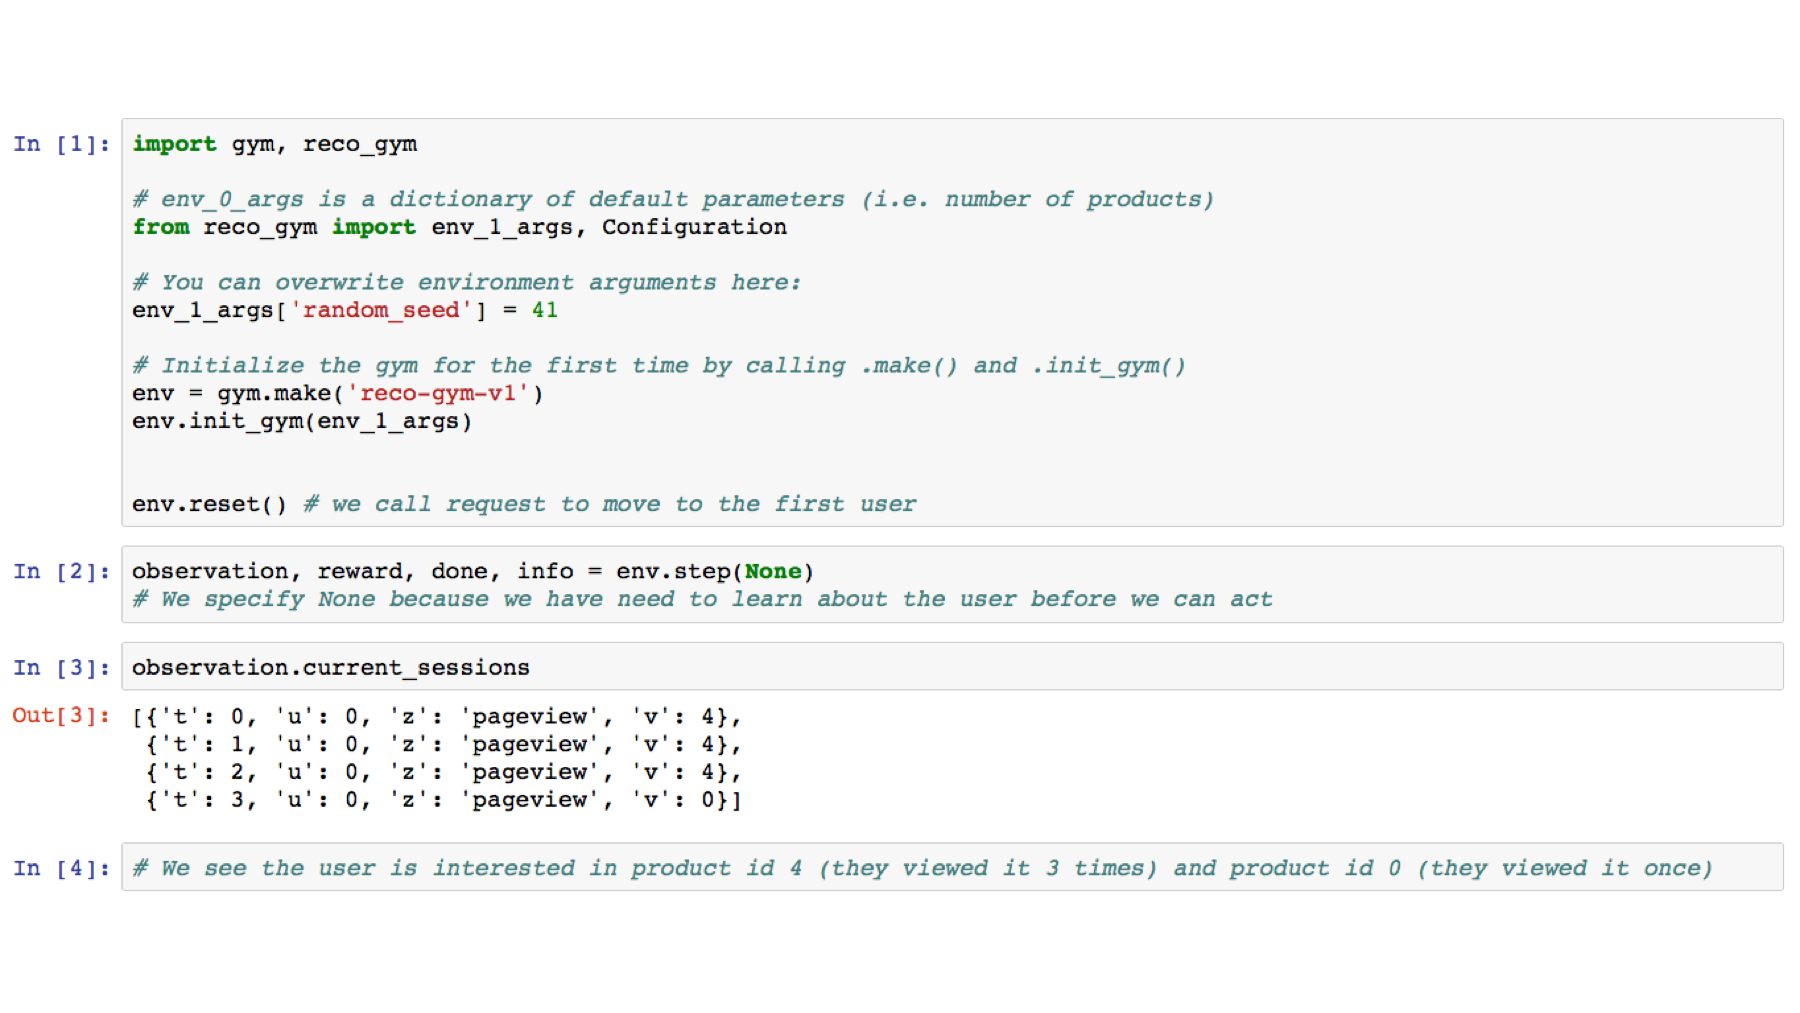
\includegraphics[scale=0.3]{images/reco_gym_sess0.png}
       \centering
       \label{motex1}
   \end{figure}
     
 \end{frame}



 \begin{frame}
  \frametitle{The RecoGym Session}
 
 
   \begin{figure}[h!]
     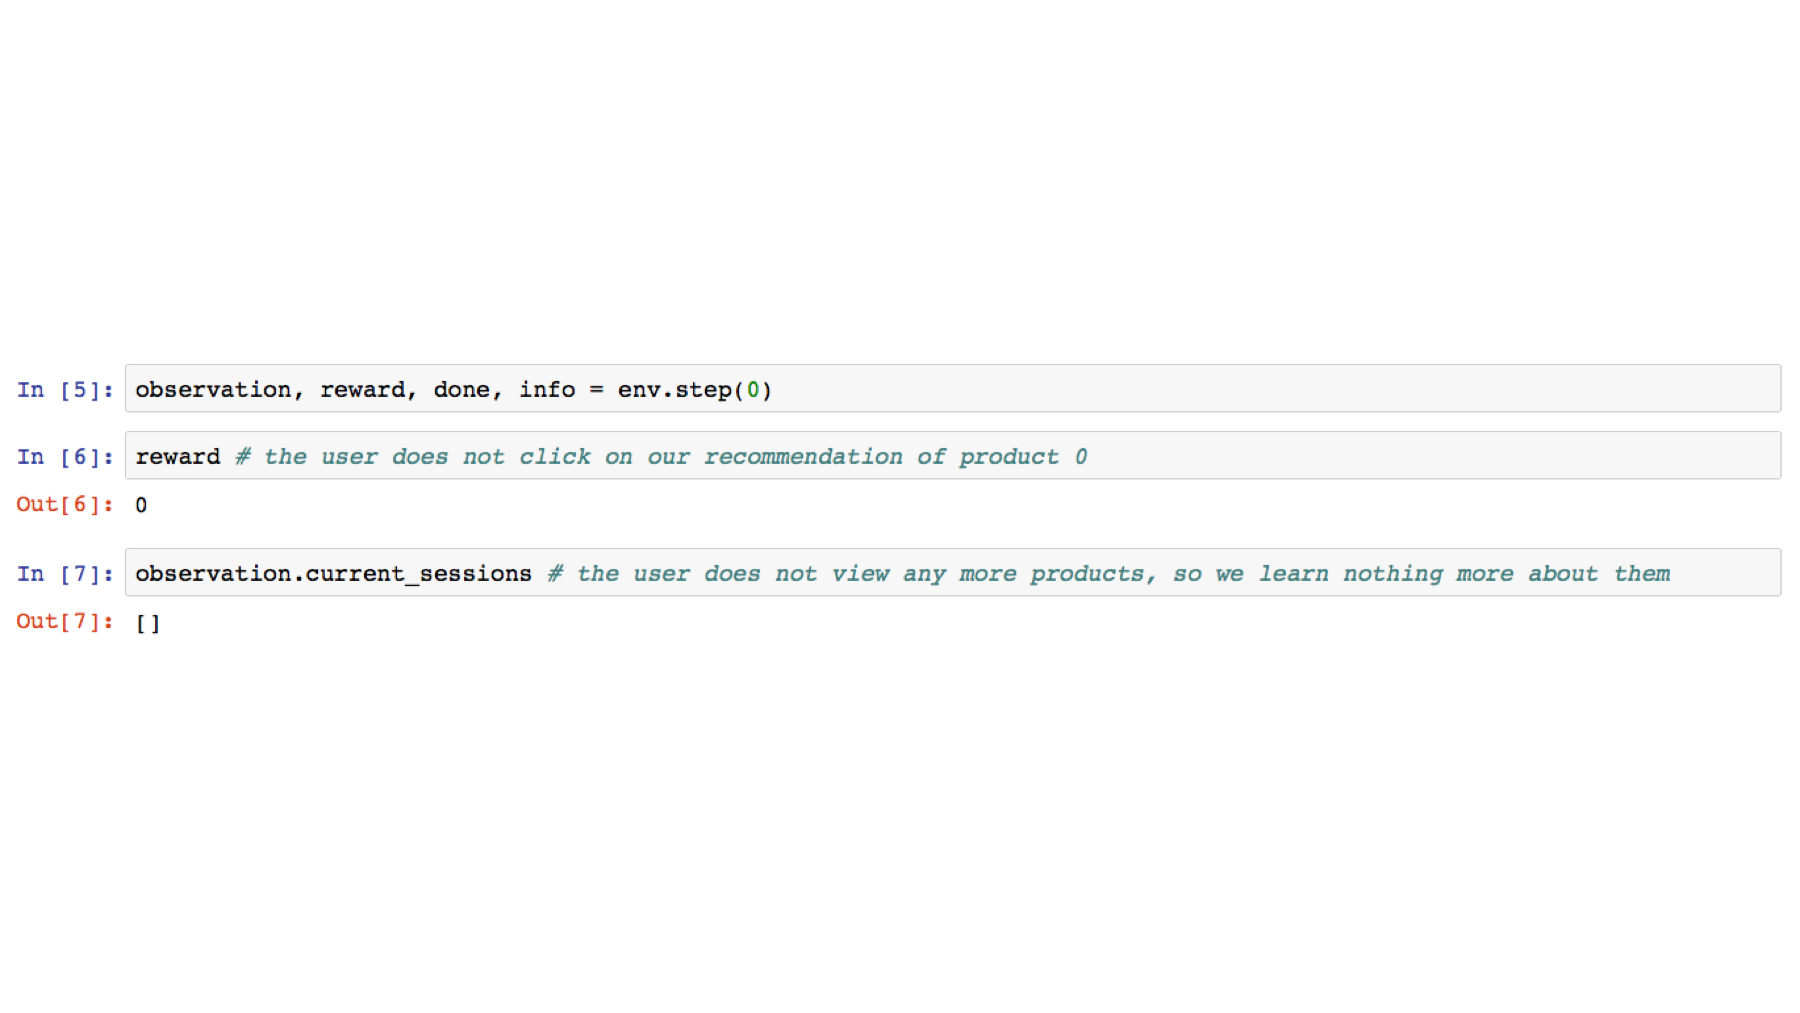
\includegraphics[scale=0.3]{images/reco_gym_sess1.png}
       \centering
       \label{motex1}
   \end{figure}
     
 \end{frame}



 \begin{frame}
  \frametitle{The RecoGym Session}
 
 
   \begin{figure}[h!]
     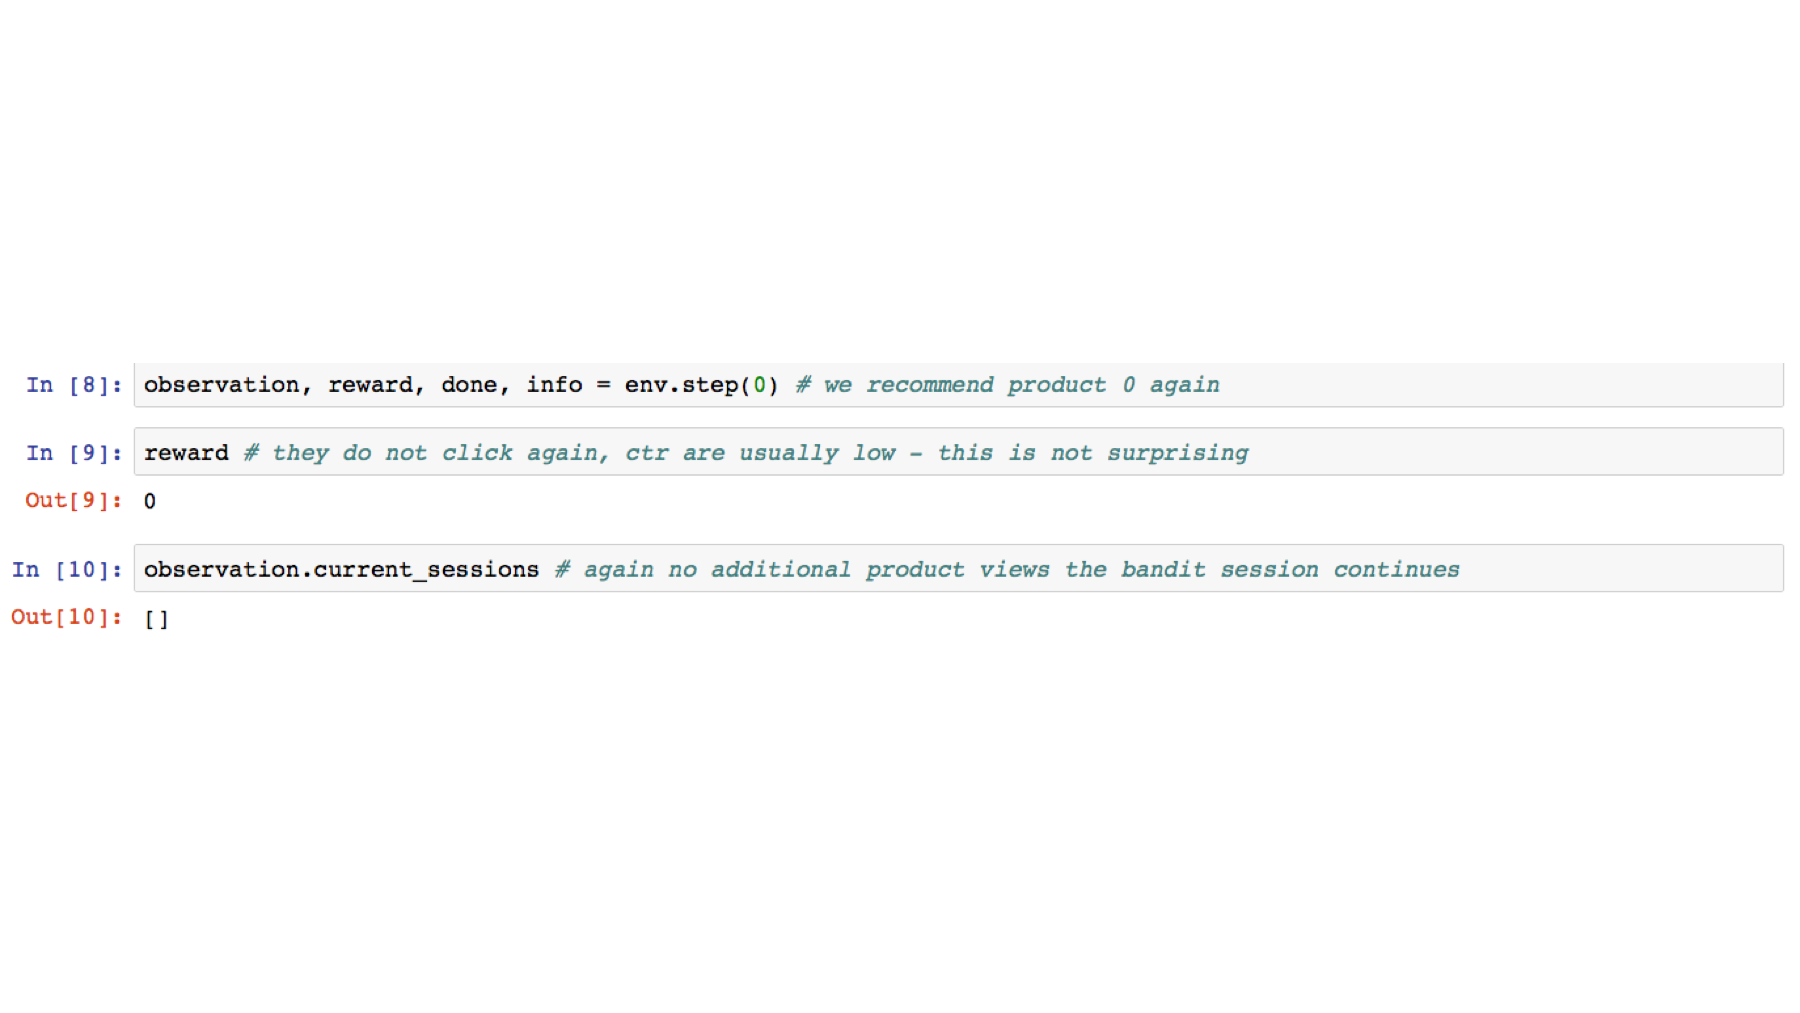
\includegraphics[scale=0.3]{images/reco_gym_sess2.png}
       \centering
       \label{motex1}
   \end{figure}
     
 \end{frame}



 \begin{frame}
  \frametitle{The RecoGym Session}
 
 
   \begin{figure}[h!]
     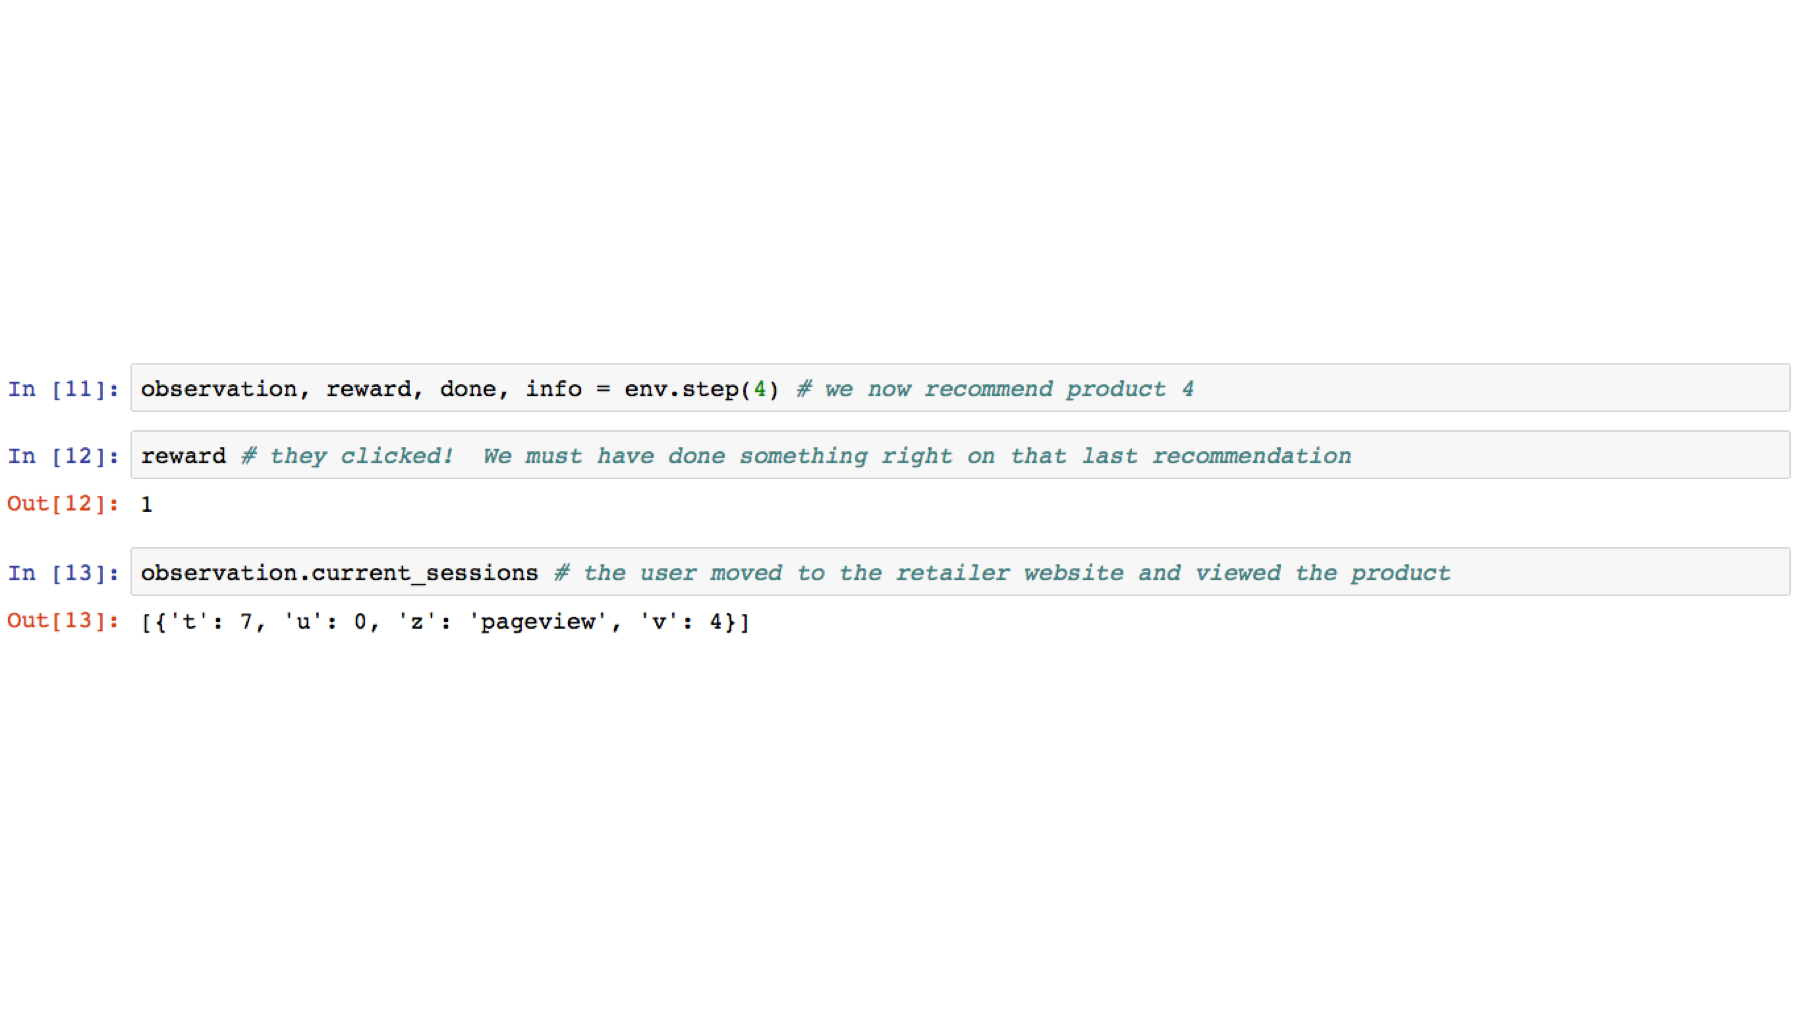
\includegraphics[scale=0.3]{images/reco_gym_sess3.png}
       \centering
       \label{motex1}
   \end{figure}
\end{frame}



   \begin{frame}
    \frametitle{Unlike RL we continue to use logs}
   
    Let's start with a random logging policy (a crazy thing to do, but a useful theoretical concept).
    
     \begin{figure}[h!]
       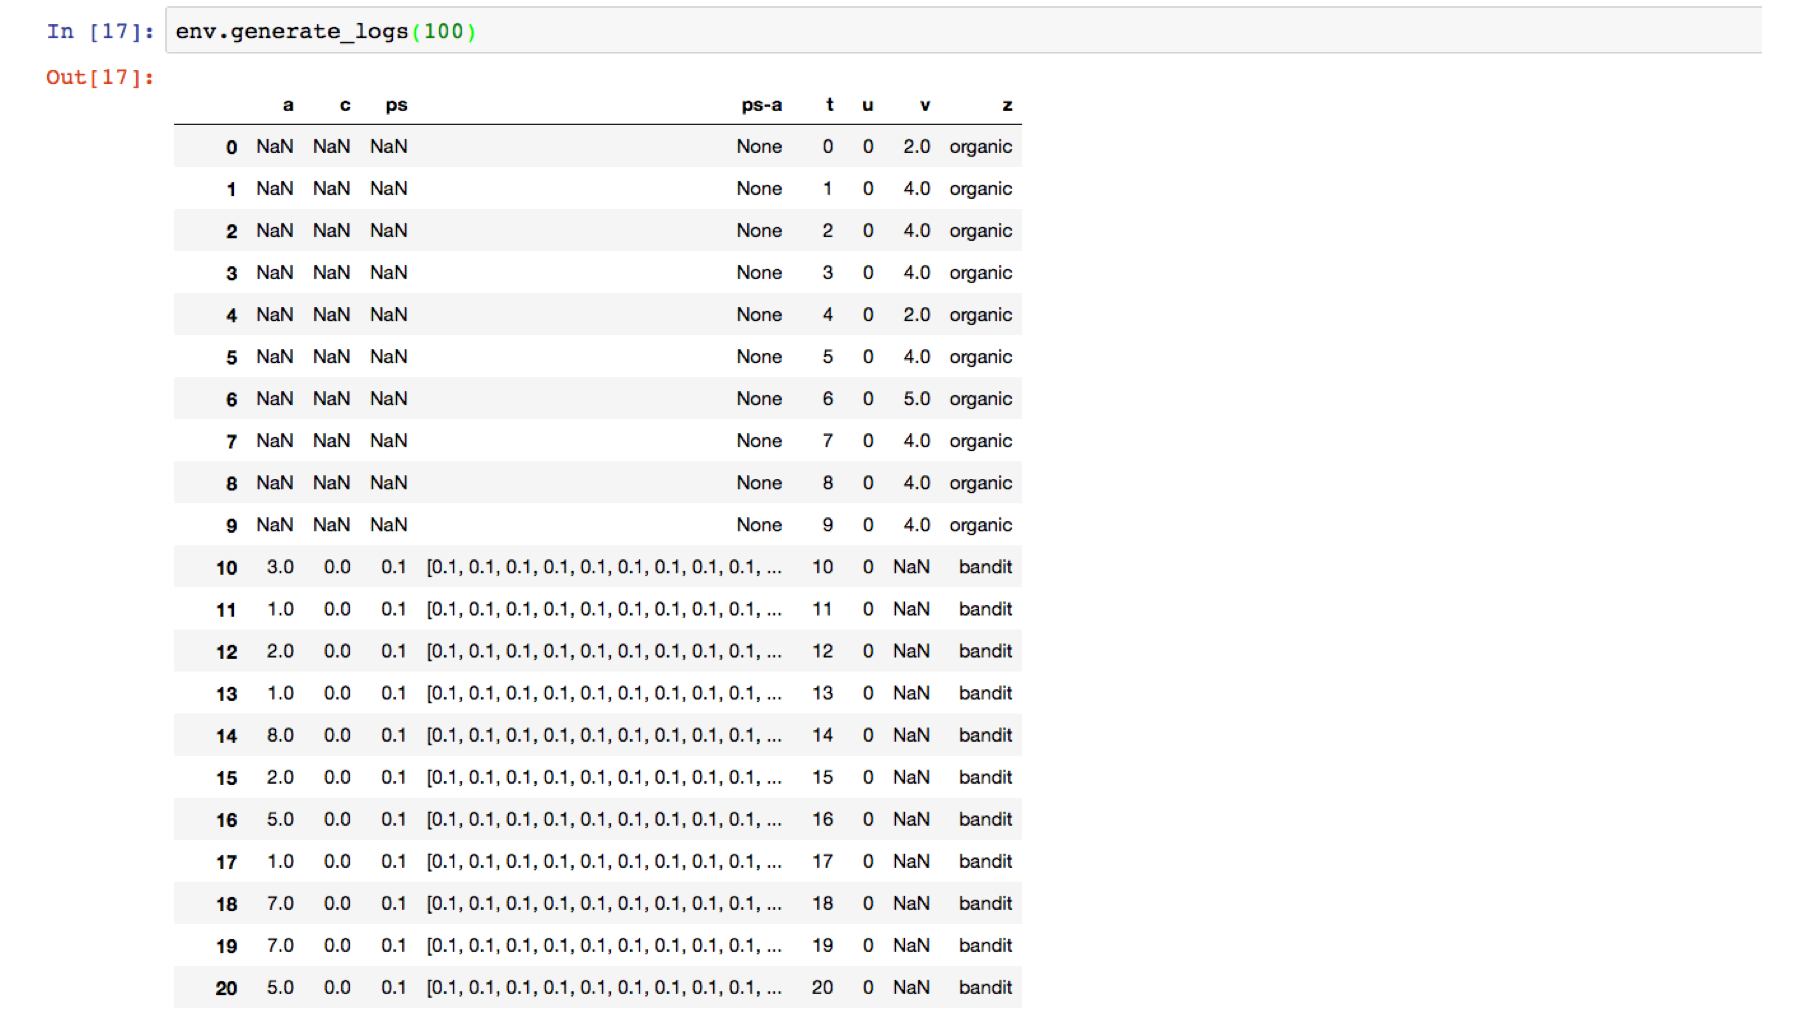
\includegraphics[scale=0.3]{images/recogymlog.png}
         \centering
         \label{motex1}
     \end{figure}
  \end{frame}

\plain{Organic Best Of vs Bandit Best Of}

  \begin{frame}
    \frametitle{Exercise - Getting Started with RecoGym}

    Go to the notebook ``Module III A.ipynb''
\begin{itemize}
  \item Examine the logs, to start with we will look at non-personalized behavior only.
  \item Plot a histogram of organic product popularity. What is the most popular product?  
  \item Plot the (non-personalized) click through rate of each product (with an error analysis).  What is the most clicked-on product?
  \item Plot popularity against click through rate.  How good a proxy is popularity for click through rate?
  \item Simulate an AB test comparing a simple recommender system (agent) that always recommends the highest ctr product with a recommender system that always recommends the organically most popular product.
\end{itemize}
\end{frame}

\begin{frame}
  \frametitle{Harder questions}

Reflect on how the logging policy would affect these results.

\pause

What is personalization? What impact does personalization bring?

\pause

Where does traditional academic recommender systems research fit into this picture?  

\end{frame}


\begin{frame}
\begin{quote}
  To consult the statistician after an experiment is finished is often merely to ask him to conduct a post mortem examination. He can perhaps say what the experiment died of.
\end{quote}
Roland Fisher
\end{frame}

\begin{frame}[fragile]
  \frametitle{Answer Q1 Histogram of product popularity}
\begin{small}
\begin{verbatim}
  clicks = np.zeros(NumberOfProducts)
  bandits = data[data['z'] == 'bandit']
  for product_id in range(NumberOfProducts):
      actions = bandits[bandits['a'] == product_id]
      clicks[product_id] = np.sum(actions[actions['c'] == 1]['c'])
      
  print("Clicks: ", clicks)
  
  _, ax = plt.subplots()
  ax.set_title('Histogram of Clicks per Product')
  
  ax.bar(range(NumberOfProducts), clicks)
  plt.show()
\end{verbatim}
\end{small}
\end{frame}


\begin{frame}[fragile]
  \frametitle{Answer Q2 Non-personalized CTR}
\begin{tiny}
\begin{verbatim}
  from scipy.stats.distributions import beta

  clicks = np.zeros(NumberOfProducts)
  impressions = np.zeros(NumberOfProducts)
  lower_errors = np.zeros(NumberOfProducts)
  upper_errors = np.zeros(NumberOfProducts)
  bandits = data[data['z'] == 'bandit']
  for product_id in range(NumberOfProducts):
      actions = bandits[bandits['a'] == product_id]
      clicks[product_id] = np.sum(actions[actions['c'] == 1]['c'])
      impressions[product_id] = sum(actions['a']==product_id)
\end{verbatim}
\end{tiny}
\end{frame}

\begin{frame}[fragile]
  \frametitle{Answer Q3 Best of CTR}
\begin{verbatim}
  top_ctr_item = np.argmax(clicks/impressions)
\end{verbatim}
\end{frame}


\begin{frame}[fragile]
  \frametitle{Answer Q4 most views}
\begin{verbatim}
  top_viewed_item = np.argmax(views)
\end{verbatim}
\end{frame}




\begin{frame}[fragile]
  \frametitle{}
  \begin{small}
\begin{verbatim}
data = deepcopy(env).generate_logs
        (ABTestNumberOfUsers, agent=organic_counter_agent)
\end{verbatim}
\end{small}
\end{frame}




\begin{frame}
\frametitle{Organic Best-Of vs Bandit Best-Of}

As the logging policy chose its actions uniformly at random, we can see that all items were recommended roughly the same number of times.

\begin{figure}[h!]
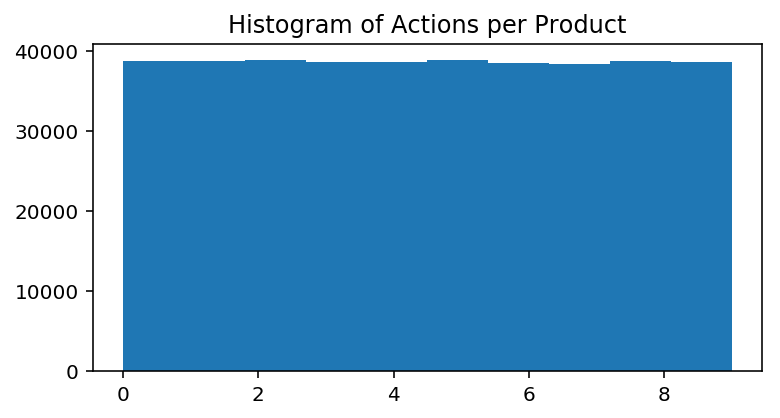
\includegraphics[scale=0.4]{images/organic_bestof0.png}
\centering
\label{motex1}
\end{figure}
\end{frame}

\begin{frame}
\frametitle{Organic Best-Of vs Bandit Best-Of}

We can examine the click through rate of each action under this policy, we see that action 5, 2 and 9 have high click through rates.

\begin{figure}[h!]
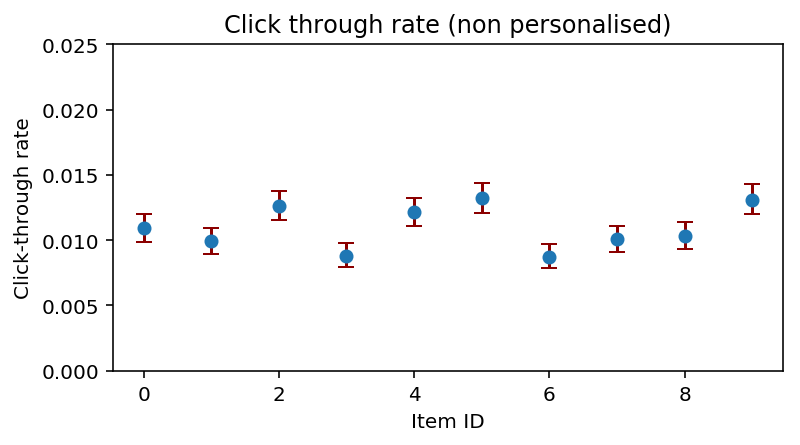
\includegraphics[scale=0.4]{images/organic_bestof1.png}
\centering
\label{motex1}
\end{figure}
\end{frame}

\begin{frame}
\frametitle{Organic Best-Of vs Bandit Best-Of}


\begin{figure}[h!]

  We can also examine which items are organically the most popular, this time we see that item 4 and item 9 are the most popular.

  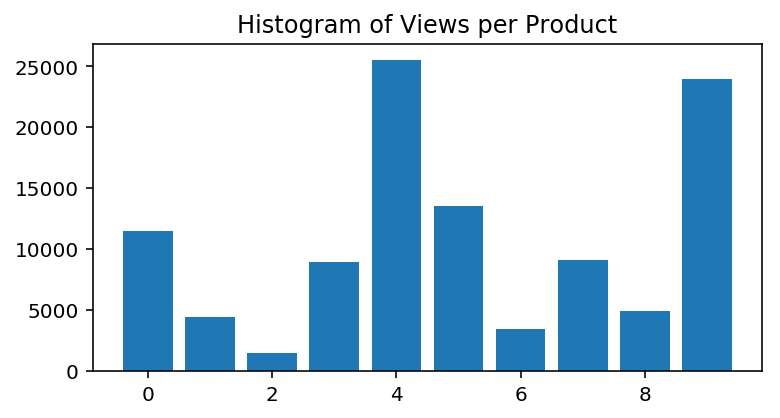
\includegraphics[scale=0.4]{images/organic_bestof2.png}
\centering
\label{motex1}
\end{figure}
\end{frame}

\begin{frame}
\frametitle{Organic Best-Of vs Bandit Best-Of}

If we plot popularity vs non-personalized click through rate we see some kind of relationship, but the correlation is noisy.


\begin{figure}[h!]
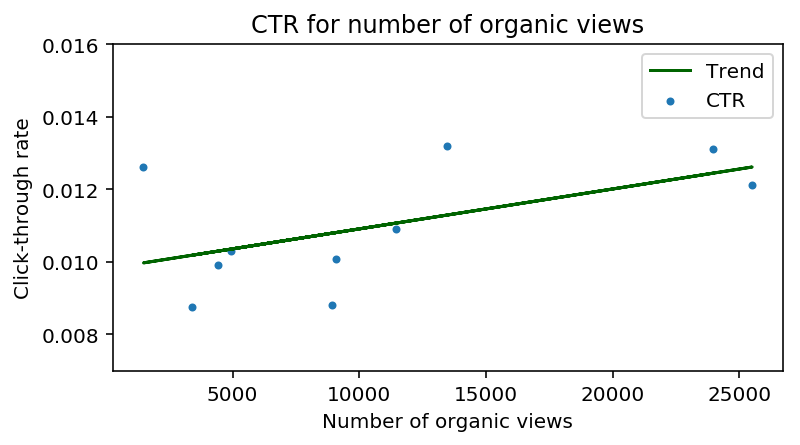
\includegraphics[scale=0.4]{images/organic_bestof3.png}
\centering
\label{motex1}
\end{figure}
\end{frame}

\begin{frame}
\frametitle{Organic Best-Of vs Bandit Best-Of}

A bandit best-of agent always recommends the highest ctr product (product 5).  An organic best-of always recommends the most frequently viewed product (product 4).  A simulated AB test shows using the bandit best-of yields a better result.

\end{frame}

\begin{frame}
\frametitle{Organic Best-Of vs Bandit Best-Of}
  
\begin{figure}[h!]
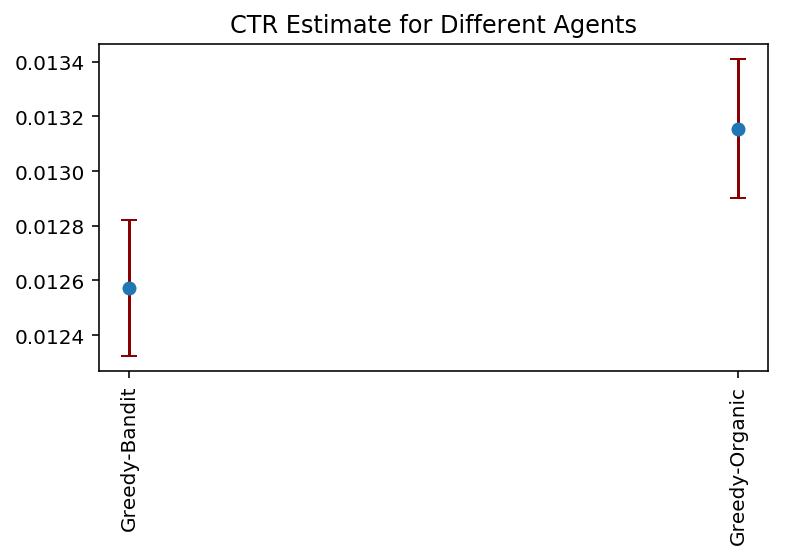
\includegraphics[scale=0.4]{images/organic_bestof4.png}
\centering
\label{motex1}
\end{figure}

\pause
Personalization of course will result in a better result still.
\end{frame}


\plain{Evaluate an organic agent using the Bandit Signal}

\begin{frame}
  \frametitle{The cold start scenario}

    \begin{itemize}
      \item You need to build a recommender system for a client, they have an existing system with existing organic traffic.  \pause This means you can build standard next item predictions to build models of user behavior and understand how user's preferences cluster together. \pause
      \item They are currently running a recommender system with a random policy. \pause
      \item Your task is to build a next item prediction model as a proxy for a recommendation algorithm.  Then produce offline metrics to convince the engineering team to run an AB test.\pause
      \item Finally you evaluate your performance against production.
    \end{itemize}

    \pause
    Please look at notebook ``Module III B.ipynb''

\end{frame}



\begin{frame}[fragile]
  \frametitle{Answer}
\begin{tiny}  
\begin{verbatim}
def observe(self, observation):
  for session in observation.sessions():
      self.user_embedding += self.embeddings[session['v'],:]
      self.history_length += 1

def act(self, observation, reward, done):
  """Act method returns an Action based on current observation and past history"""
  self.observe(observation)
  next_item_score = np.matmul(self.embeddings,self.user_embedding/self.history_length)

  action = np.argmax(next_item_score)        
  prob = np.zeros_like(next_item_score)
  prob[action]=1.0
  return {
      **super().act(observation, reward, done),
      **{
          'a': action,
          'ps': 1.0,
          'ps-a': prob,
      },
  }
\end{verbatim}
\end{tiny}
\end{frame}




\begin{frame}
  \frametitle{Evaluate an organic model using Bandit Feedback}

  Methods like word2vec and SVD can be used to produce a low rank factorization of a matrix of co-counts.  Imagine we have 500 products and we have observed the co-counts on the right, the matrix on the left can produce a good reconstruction (perhaps better than the original as it can fill in missing signal).  It also uses less parameters, which has both computational and statistical advantages.

  You could also use deep learning (see modules 1 and 2 of our course)

  \begin{figure}[h!]
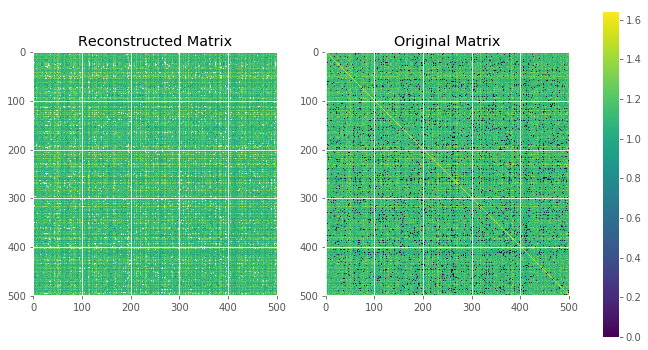
\includegraphics[scale=0.4]{images/evalorganicwithbandit0.png}
\centering
\label{motex1}
\end{figure}
\end{frame}


\begin{frame}
  \frametitle{Evaluate an organic model using Bandit Feedback}
\begin{figure}[h!]
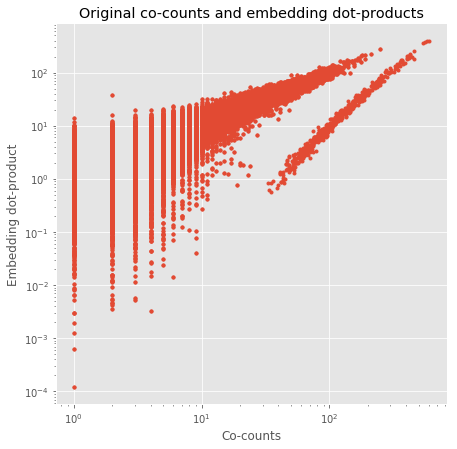
\includegraphics[scale=0.4]{images/evalorganicwithbandit1.png}
\centering
\label{motex1}
\end{figure}
\end{frame}


\begin{frame}
  \frametitle{Evaluate an organic model using Bandit Feedback}

  For such an organic method, a standard metric is hitrate-at-5 (HR@5) also called Recall@5 or Precision@5.
\begin{figure}[h!]
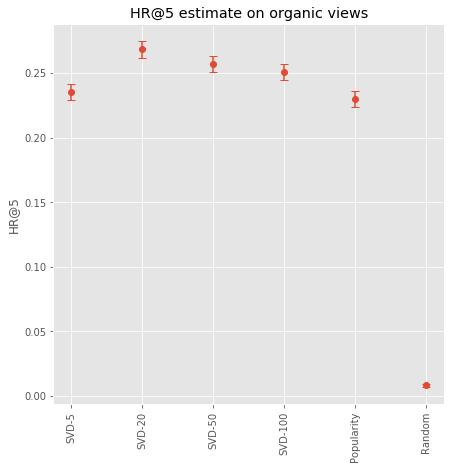
\includegraphics[scale=0.4]{images/evalorganicwithbandit2.png}
\centering
\label{motex1}
\end{figure}
\end{frame}

\begin{frame}
  \frametitle{Evaluate an organic model using Bandit Feedback: IPS evaluation}

Hit-rate is a purely organic measure that is available offline and is seen in many recommender systems papers...  \pause but it is a purely organic metric, it doesn't predict performance at AB test time, at least not explicitly.

\pause

Can we change to an offline measure that predicts the result of an AB test?

\pause

Imagine the past policy is randomized, i.e. with some probability it will choose any action for a given user.  \pause Random isn't the same as uniform and the policy typically will not be uniformly random. \pause \emph{Why?} \pause ... still, a uniformly random logging policy is an interesting thought experiment or reference.

\end{frame}

\begin{frame}
  \frametitle{Evaluate an organic model using Bandit Feedback: IPS evaluation}

The central idea of an inverse propensity score is that we evaluate a new policy using the logs of an old policy.  \pause We identify times in history where the new policy would make the same recommendation as the old policy, we then look at the contribution of the reward and how probable the policy is to take this action. 

\[
\text{CTR}_{\pi_t}(\mathcal{L}) = \frac{1}{|\mathcal{L}|}\sum_{(a,x,c) \in \mathcal {L}} c \frac{\pi_t(a|x)}{\pi_l(a|x)}
\]

\end{frame}


\begin{frame}
  \frametitle{Evaluate an organic model using Bandit Feedback}
\begin{figure}[h!]
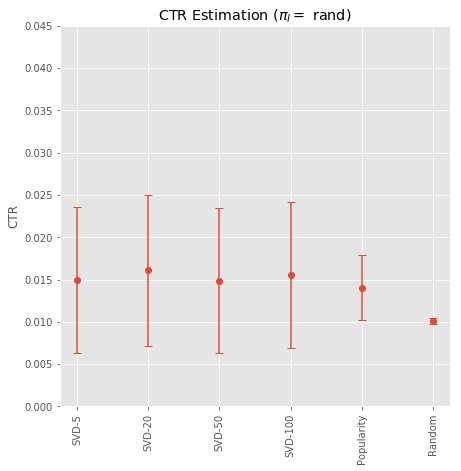
\includegraphics[scale=0.4]{images/evalorganicwithbandit3.png}
\centering
\label{motex1}
\end{figure}
\end{frame}

\begin{frame}
  \frametitle{Evaluate an organic model using Bandit Feedback}
\begin{figure}[h!]
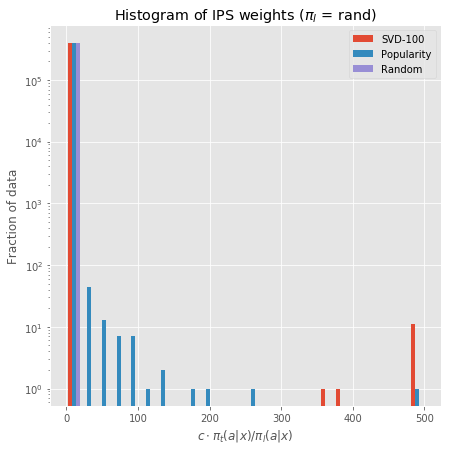
\includegraphics[scale=0.4]{images/evalorganicwithbandit4.png}
\centering
\label{motex1}
\end{figure}
\end{frame}

\begin{frame}
  \frametitle{Evaluate an organic model using Bandit Feedback}
\begin{figure}[h!]
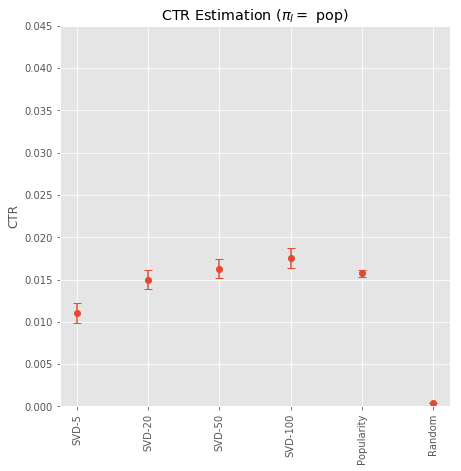
\includegraphics[scale=0.4]{images/evalorganicwithbandit5.png}
\centering
\label{motex1}
\end{figure}
\end{frame}

\begin{frame}
  \frametitle{Evaluate an organic model using Bandit Feedback}
\begin{figure}[h!]
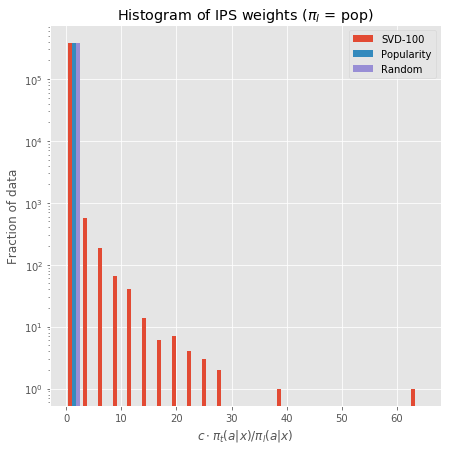
\includegraphics[scale=0.4]{images/evalorganicwithbandit6.png}
\centering
\label{motex1}
\end{figure}
\end{frame}


\begin{frame}
  \frametitle{Evaluate an organic model using Bandit Feedback: Simulated A/B-Test Results}
\begin{figure}[h!]
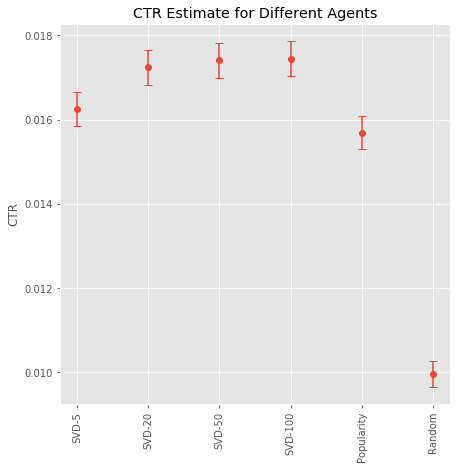
\includegraphics[scale=0.4]{images/evalorganicwithbandit7.png}
\centering
\label{motex1}
\end{figure}
\end{frame}


\plain{LIkelihood Based Agents}

\begin{frame}
  \frametitle{Likelihood Based Agent}

  \[
    c_n \sim {\rm Bernoulli}
      \left(
        \sigma
          \left(
      \bPhi {\left( [\bX_n ~ \ba_n] \right)}^T \bbeta
          \right)
      \right)
    \]

    where
    \begin{itemize}
      \item $\bbeta$ are the parameters;
      \item $\sigma \left( \cdot \right)$ is the logistic sigmoid;
      \item $\bPhi \left( \cdot \right)$ is a function that maps $\bX,\ba$ to a higher dimensional space and includes some interaction terms between ${\bX}_n$ and ${\ba}_n$. \pause \emph{Why?}
    \end{itemize}
    


\end{frame}

\begin{frame}
  \frametitle{Likelihood Based Agent}

Or using $\bPhi \left( \left[ {\bX}_n ~ {\ba}_n \right] \right) = {\bX}_n \otimes {\ba}_n$:

\begin{align*}
	\hat{\bbeta}_{\rm lh} = {\rm argmax}_{\bbeta}
	& \sum_n c_n \log \sigma
				\left(
					{
						\left(
							{\bX}_n \otimes {\ba}_n
						\right)
					}^T \bbeta
				\right) \\
	& + \left(
		1-c_n
	  \right)
	  \log
	  \left(
	  	1 - \sigma
			\left(
				{
					\left(
						{\bX}_n \otimes {\ba}_n
					\right)
				}^T \bbeta
			\right)
	\right)
  \end{align*}
\end{frame}


\begin{frame}
  \frametitle{Feature Engineering to get the context vector $\bX$}

  The above model requires us to specify the context $\bX$, how can we do this?
\end{frame}



\begin{frame}
  \frametitle{Feature Engineering}
\begin{figure}[h!]
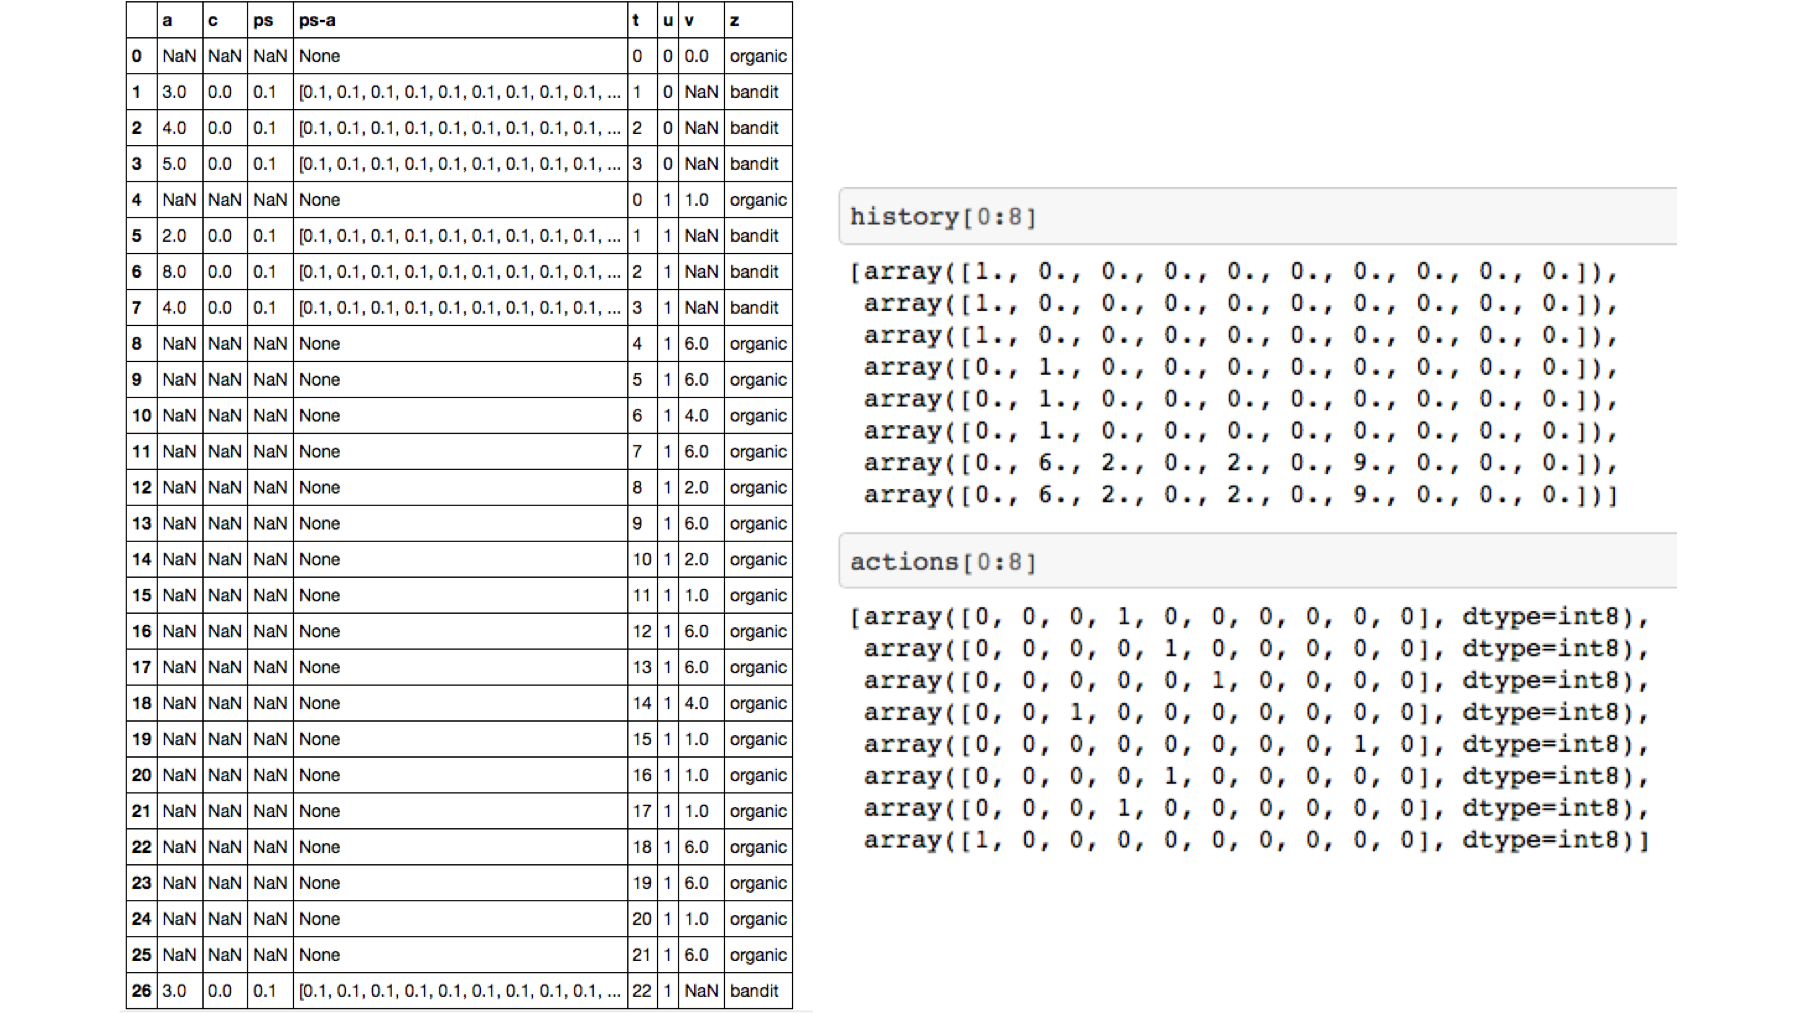
\includegraphics[scale=0.3]{images/feature_engineering.png}
\centering
\end{figure}

\pause
How would you interact the features?

\pause
Is this a good feature engineering scheme?  Can you improve it?
\end{frame}


\begin{frame}
  \frametitle{Other ways to train on bandit feedback - reweighted likelihood}

  What if we fit an overly simplified parametric model to the data?
  \pause

  The simple model will predict accurately for the most frequent actions and compromise the fit for the least frequent actions.


\begin{align*}
	\hat{\bbeta}_{\operatorname{re-weight}} =  {\rm argmax}_{\bbeta}
	\sum_n
	& w_n c_n \log \sigma
		\left(
			{\bPhi
				\left(
					\left[ {\bX}_n ~ {\ba}_n \right]
				\right)
			}^T \bbeta
		\right)  \\
	& + w_n \left( 1-c_n \right)
		\log
			\left(
				1 - \sigma
					\left(
						{\bPhi \left(
								\left[ {\bX}_n ~ {\ba}_n \right]
							\right)
						}^T \bbeta
					\right)
			\right)
\end{align*}

where the weight is defined: $w_n = \frac{1}{\pi\left( {\ba}_n | {\bX}_n \right)}$.

\end{frame}


\begin{frame}
  \frametitle{Pure Organic vs Pure Bandit}
\begin{figure}[h!]
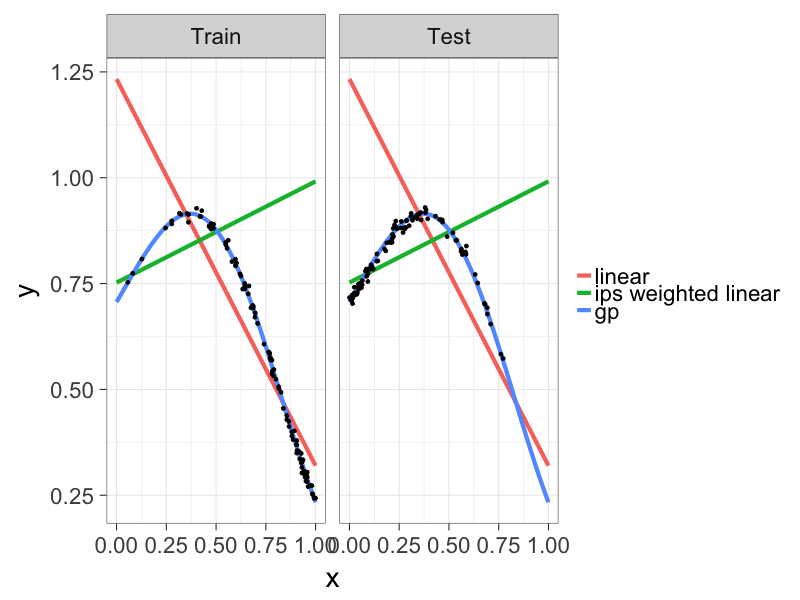
\includegraphics[scale=0.4]{images/two_linear_models_and_gp5.png}
\centering
\end{figure}
\end{frame}


\begin{frame}
  \frametitle{Other ways to train on bandit feedback - counterfactual risk}

  Often in machine learning we search for a decision rule that would have worked well in the past.  \pause We call this empirical risk.

  \pause

  We can't evaluate decisions we didn't do in the past.  \pause We can however use IPS to estimate them.

  \pause

  A direct estimation of this leads to the contextual bandit formulation:

  \pause


  \[
    \pi_{\bbeta}\left( {\ba}_n | {\bX}_n \right) = {\rm softmax}
      \left( {\bPhi
        \left(
          \left[ \bX_n ~ \ba_n \right]
        \right)}^T \bbeta
      \right)
  \]  

\end{frame}


\begin{frame}
  \frametitle{Other ways to train on bandit feedback - counterfactual risk}

\begin{align*}
	\hat{\bbeta}_{\rm CB} = {\rm argmax}_{\bbeta} \sum_n
	& w_n c_n
		{\left(
			{\bX}_n \otimes {\ba}_n
		\right)}^T ~ \bbeta \\
	& - w_n c_n \log \sum_{{\ba}_{n}^{'}} e^{
						{\left(
							{\bX}_n \otimes {\ba}_{n}^{'}
						\right)}^T \bbeta
						} \\
\end{align*}

\end{frame}



\begin{frame}
  \frametitle{Three methods}
\begin{figure}[h!]
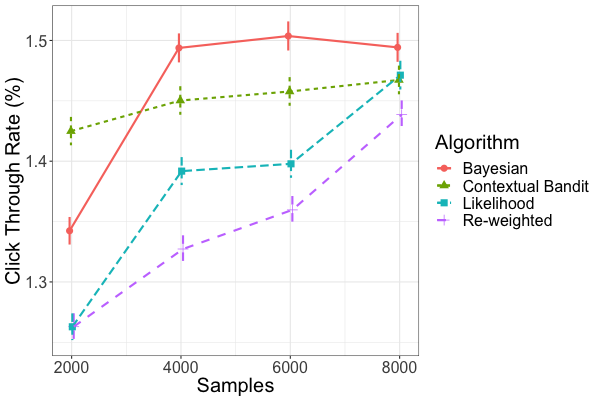
\includegraphics[scale=0.45]{images/pop_sampling_run.png}
\centering
\end{figure}


\end{frame}



\begin{frame}
  \frametitle{Three methods}
\begin{figure}[h!]
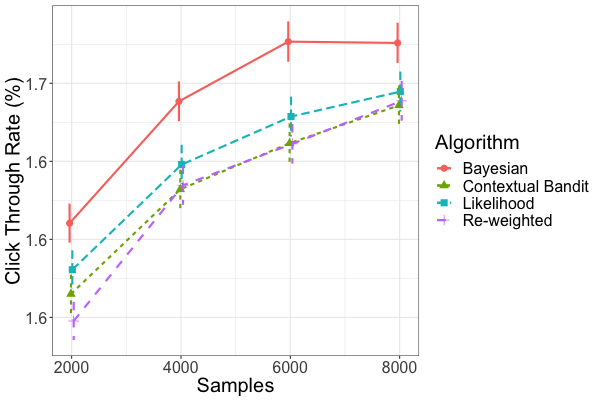
\includegraphics[scale=0.45]{images/inv_pop_sampling_run.png}
\centering
\end{figure}

Much more in the next moudule.  For a short summary see our paper: ``Three methods for training on Bandit feedback''

\end{frame}





\plain{Combining Organic Signal with Bandit Signal}


\begin{frame}
  \frametitle{Pure Organic vs Pure Bandit}
\begin{figure}[h!]
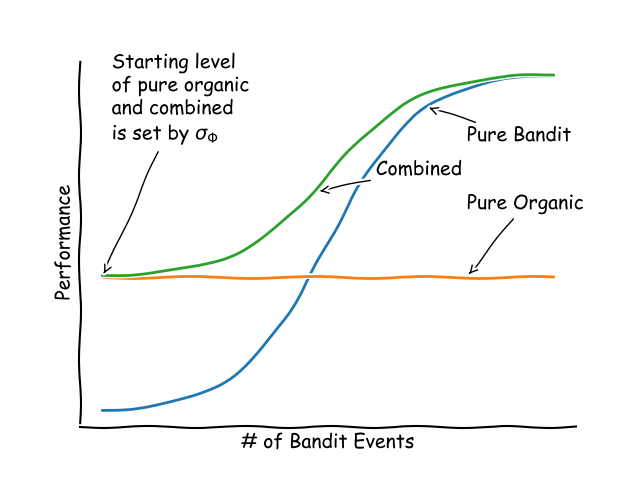
\includegraphics[scale=0.45]{images/pureorganicpurebandit.png}
\centering
\end{figure}
\end{frame}






\begin{frame}
  \frametitle{Can we get the best of both worlds?}

A simple algorithm:

\pause
Use one of the methods from the first part of the course on the organic data to prouduce product embeddings.  Classic methods are SVD or word2vec.

\pause

A user's history is then a list of embeddings rather than non-descript identifiers.

\pause

The action space is also in the same embedding space.

\pause

Exercise: implement this approach.  See ``INSERT NAME''

\pause

\emph{What advantages or challenges do you have in this approach?}
\end{frame}
